% =============================================================
% paper/main.tex —— 论文入口（只做结构组装，正文一律在 sections/）
% 编译：latexmk -xelatex -interaction=nonstopmode -halt-on-error -cd -outdir=build paper/main.tex
% 注意：正文一个字都不要写在本文件（共享文件，冲突高发）。
%
% 版式依据 problem/format2026.doc（2026 年修订稿）：
%   第三条 摘要页单独一页，页码位于页脚中部、从摘要页起用阿拉伯数字连续编号；
%   第四条 正文从第 4 页开始、不含目录、不超过 30 页；正文之后是附录（页数不限）。
% =============================================================
\documentclass[12pt,a4paper]{ctexart}

% =============================================================
% paper/preamble.tex —— 论文全局宏包、格式、符号宏、自定义命令
% 唯一真源：docs/NOTATION.md（符号）、paper/refs.bib（参考文献）
% 编译方式：XeLaTeX（latexmk -xelatex），严禁 pdflatex（中文会炸）
% =============================================================

% ---------- 页面设置（数模论文常规 2.5cm 页边距） ----------
\usepackage[a4paper,margin=2.3cm,top=2.4cm,bottom=2.4cm]{geometry}

% ---------- 数学 ----------
\usepackage{amsmath}
\usepackage{amssymb}
\usepackage{bm}   % 向量/矩阵加粗用 \bm

% ---------- 表格（一律 booktabs 三线表，禁用竖线） ----------
\usepackage{booktabs}
% 论文含十余张表与十余幅图，统一收紧浮动体间距以控制篇幅
\setlength{\floatsep}{4pt plus 1pt minus 1pt}
\setlength{\textfloatsep}{6pt plus 1pt minus 1pt}
\setlength{\intextsep}{5pt plus 1pt minus 1pt}
\setlength{\abovecaptionskip}{3pt}
\setlength{\belowcaptionskip}{0pt}
% 放宽浮动体页面配额：本文含 15 幅图与 17 张表，若限制过严会在页面底部留下大片空白
\renewcommand{\topfraction}{0.92}
\renewcommand{\bottomfraction}{0.75}
\renewcommand{\textfraction}{0.08}
\renewcommand{\floatpagefraction}{0.80}
\setcounter{topnumber}{3}
\setcounter{bottomnumber}{2}
\setcounter{totalnumber}{4}
\usepackage{longtable}  % 跨页符号表
\usepackage{multirow}
% 假设条目：不依赖 enumitem 的可选参数（曾被 enit@postlabel 的括号陷阱绊住），
% 直接用零间距自定义环境，保证任何 TeX 发行版下都能编译。
\newenvironment{assumptionlist}{%
  \begin{list}{}{\setlength{\leftmargin}{2.4em}\setlength{\labelwidth}{2.0em}%
    \setlength{\labelsep}{0.4em}\setlength{\itemindent}{0pt}%
    \setlength{\itemsep}{1pt}\setlength{\parsep}{0pt}\setlength{\topsep}{2pt}}%
}{\end{list}}
\usepackage{array}
\usepackage{graphicx}   % \resizebox 用于超宽表格

% ---------- 颜色（xcolor 需早于 listings 加载） ----------
\usepackage{xcolor}

% ---------- 插图 ----------
\graphicspath{{figs/}}

% ---------- 流程图与示意图（TikZ；不依赖外部图片文件） ----------
\usepackage{tikz}
\usetikzlibrary{arrows.meta,positioning,shapes.geometric,fit,backgrounds,calc}
\tikzset{
  box/.style={draw, rounded corners=2pt, align=center, font=\small,
              minimum height=7mm, inner sep=2.4pt, fill=blue!4},
  data/.style={box, fill=green!8},
  phys/.style={box, fill=orange!10},
  num/.style={box, fill=blue!8},
  deliv/.style={box, fill=purple!8},
  ver/.style={box, fill=red!7},
  flow/.style={-{Latex[length=2mm]}, thick},
  note/.style={font=\scriptsize, align=left, text=black!70},
}

% ---------- 代码（Python 样式；统一 UTF-8，XeLaTeX 下中文正常） ----------
\usepackage{listings}
\lstset{
  language=Python,
  basicstyle=\ttfamily\scriptsize,
  extendedchars=true,
  inputencoding=utf8,
  showstringspaces=false,
  columns=fullflexible,
  keepspaces=true,
  frame=single,
  framexleftmargin=2pt,
  breaklines=true,
  breakatwhitespace=false,
  postbreak=\mbox{\textcolor{gray}{$\hookrightarrow$}\space},
  commentstyle=\color{gray},
  keywordstyle=\color{blue!60!black},
  stringstyle=\color{orange!80!black},
  numbers=left,
  numberstyle=\tiny\color{gray},
  tabsize=4,
}

% ---------- 数学单位（siunitx v3 语法：\qty{}{} 与 \unit{}，勿用 v2 的 \SI{}{}） ----------
\usepackage{siunitx}
\sisetup{per-mode=symbol, detect-all}

% ---------- 算法（algorithm2e；备选 algorithm+algpseudocode，二选一勿同开） ----------
\usepackage[linesnumbered,ruled]{algorithm2e}

% ---------- 参考文献（GB/T 7714 数字顺序制，中国数模论文通用格式） ----------
% main.tex 用 \bibliographystyle{gbt7714-numerical} + \bibliography{refs}。
\usepackage[sort&compress]{natbib}
\bibliographystyle{gbt7714-numerical}
\setcitestyle{super,comma}   % 上标数字引用，正文用 \cite{...}
\renewcommand{\bibfont}{\small}

% ---------- 超链接与交叉引用（hyperref 必须最后加载，cleveref 在其之后） ----------
\usepackage[hidelinks,bookmarksnumbered=true]{hyperref}
\hypersetup{
  pdftitle={圆柱形中药材热风烘干过程的传热-传质耦合模型},
  pdfauthor={},
}
\usepackage[nameinlink]{cleveref}

% =============================================================
% 符号宏（唯一真源：docs/NOTATION.md §0「三层命名映射」）
% 规则：论文里不要直接写 $T$，要写 \T；改名只改这一处，全文自动同步。
% 说明：\t 覆盖 LaTeX 原生的 tie 重音（\renewcommand）；
%       r/k/h/L/D 等常用简写已按 NOTATION.md 规避：
%       r→\rpos、k→\kcond、h→\hconv、L→\Llen、D→\Ddiff。
% =============================================================
\renewcommand{\t}{\ensuremath{t}}           % 时间
\newcommand{\T}{\ensuremath{T}}             % 药材温度
\newcommand{\C}{\ensuremath{C}}             % 水分浓度（干基含水率）
\newcommand{\rpos}{\ensuremath{r}}          % 到药材中心的径向距离
\newcommand{\R}{\ensuremath{R}}             % 药材半径（问题 4 中随时间变化）
\newcommand{\Rzero}{\ensuremath{R_0}}       % 初始半径
\newcommand{\Llen}{\ensuremath{L}}          % 药材长度
\newcommand{\cp}{\ensuremath{c_p}}          % 定压比热容
\newcommand{\kcond}{\ensuremath{k}}         % 导热系数
\newcommand{\Ddiff}{\ensuremath{D}}         % 水分扩散系数
\newcommand{\hconv}{\ensuremath{h}}         % 对流换热系数
\newcommand{\hmass}{\ensuremath{h_m}}       % 对流传质系数
\newcommand{\Tinf}{\ensuremath{T_\infty}}   % 烘房（环境）温度
\newcommand{\Cinf}{\ensuremath{C_\infty}}   % 烘房（环境）水分浓度
\newcommand{\wfrac}{\ensuremath{w}}         % 水分质量分数 w = C/(1+C)
\newcommand{\dt}{\ensuremath{\Delta t}}     % 时间步长
\newcommand{\dr}{\ensuremath{\Delta r}}     % 空间步长
\newcommand{\Nr}{\ensuremath{N_r}}          % 径向网格节点数
\newcommand{\tend}{\ensuremath{t_{\mathrm{end}}}}  % 烘干结束时刻
% （\rho、\xi 为 LaTeX 原生，无需定义）

% =============================================================
% 自定义命令
% =============================================================
% \instruction{...}：醒目的 TODO 占位提示（待填内容用）
\newcommand{\instruction}[1]{%
  \par\medskip\noindent
  \fcolorbox{orange!70!black}{orange!10}{%
    \parbox{\dimexpr\linewidth-2\fboxsep-2\fboxrule}{%
      \textbf{\textcolor{orange!60!black}{【TODO 占位】}}\, #1}}%
  \par\medskip
}

% \code{...}：行内代码
\newcommand{\code}[1]{\texttt{#1}}

% \geninput{tab/foo}{补充说明}：安全引入由 scripts 生成的片段。
% 依据 AGENTS.md 铁律 10「不许静默降级」：片段缺失时**不静默跳过**，
% 而是打印醒目的占位框，让缺表在 PDF 里一眼可见。
% \detokenize 把路径中的下划线还原为普通字符 —— 否则"文件缺失"提示本身
% 会因为 \texttt{tab/foo_bar} 里的下划线进入数学模式而报错（实测踩过）。
\newcommand{\geninput}[2]{%
  \IfFileExists{#1.tex}{%
    \input{#1}%
  }{%
    \instruction{【生成产物缺失】未找到 \texttt{\detokenize{#1}.tex}。#2
      请先运行 \texttt{make tables}（表格与数值宏）或 \texttt{make figs}（插图）。}%
  }%
}

% \genfig[宽度]{figs/xxx.pdf}{题注}{label}：安全插图（缺文件时打印占位框）
\newcommand{\genfig}[4][0.48\linewidth]{%
  \begin{figure}[!ht]
    \centering
    \IfFileExists{#2}{%
      \includegraphics[width=#1]{#2}%
    }{%
      \instruction{【插图缺失】未找到 \texttt{\detokenize{#2}}。请先运行 \texttt{make figs}。}%
    }%
    \caption{#3}\label{#4}%
  \end{figure}%
}

% \genfigwide{...}：整幅宽度（宽图专用）
\newcommand{\genfigwide}[3]{%
  \begin{figure}[!ht]
    \centering
    \IfFileExists{#1}{%
      \includegraphics[width=\linewidth]{#1}%
    }{%
      \instruction{【插图缺失】未找到 \texttt{#1}。请先运行 \texttt{make figs}。}%
    }%
    \caption{#2}\label{#3}%
  \end{figure}%
}

% 数值宏：由 make tables 从 results/ 生成，缺失时显示 ?? 而不是编译中断
\newcommand{\genvalues}[1]{%
  \IfFileExists{tab/#1.tex}{\input{tab/#1}}{%
    \PackageWarning{paper}{tab/#1.tex 缺失，对应数值宏显示为 ??}%
  }%
}
\newcommand{\qonevalues}{\genvalues{q1_values}}
\newcommand{\qallvalues}{\genvalues{problem_values}}

% 关键词（若 ctexart 已定义则不覆盖）
\providecommand{\keywords}[1]{%
  \par\medskip\noindent\textbf{关键词：}#1\par}

% =============================================================
% 版式：摘要独占一页；正文页码从摘要页起为 1（format2026.doc 第三条）
% =============================================================
\setlength{\parskip}{1pt}
\linespread{0.98}
\ctexset{
  section/format = \raggedright\bfseries\zihao{4},
  subsection/format = \raggedright\bfseries\zihao{-4},
  subsubsection/format = \raggedright\bfseries\zihao{-4},
}
% 参考文献标题用「参考文献」而不是「References」
\renewcommand{\refname}{参考文献}


\title{\bfseries 圆柱形中药材热风烘干过程的传热--传质耦合模型\\[2pt]
       \large ——基于材料坐标移动边界与自适应隐式积分的四问统一求解}
\author{}
\date{}

\begin{document}
% 结果数值宏（由 make tables 从 results/ 生成；缺失时显示为 ??）
\qonevalues
\qallvalues

% ---- 摘要页：页码从本页开始编号（阿拉伯数字 1） ----
\pagenumbering{arabic}
\setcounter{page}{1}
\pagestyle{plain}

\maketitle

\vspace{-1.2em}
\begin{abstract}
针对圆柱药材预热、恒温干燥及失水收缩过程，建立一维轴对称热质耦合模型。四问均在表面热平衡中计入实际水分通量乘汽化潜热，并区分药材干基含水率与空气湿度比，以内部供水能力和气膜传质能力共同限制蒸发。物性严格分别采用题给附录2、3、4；通过材料坐标变换处理收缩并保持干物质量守恒，以有限体积法和BDF隐式积分求解。

问题一使用附件实测环境，1800~s时中心、表面温度分别为\QOneCenterT{}、\QOneSurfaceT{}~$^\circ$C，含水率分别为\QOneCenterC{}、\QOneSurfaceC{}~kg/kg。问题二建立全程变物性模型，前4~h保留附件输入，后续主方案依据文献选择\EnvTempC{}~$^\circ$C、\EnvRHPercent{}\%相对湿度；3~h时中心温度为\QTwoCenterT{}~$^\circ$C、含水率为\QTwoCenterC{}~kg/kg。

问题三以全域最大含水率低于0.15~kg/kg为判据，得到连续达标时长\QThreeEndH{}~h。问题四结合实测半径及附录4物性，得到\QFourEndH{}~h，终点半径\QFourEndRadiusCm{}~cm。另对附件升温曲线拟合渐近温度，构造\FitTempC{}~$^\circ$C、20\%相对湿度的第二方案，其问题三、四时长分别为\FitQThreeEndH{}、\FitQFourEndH{}~h；该温度依赖外推模型，不能视为已观测到的稳态。

对新模型开展空间加密、时间积分交叉、守恒收支及工况对照，并生成四个完整结果工作簿。药材种类与解吸数据缺失导致表面供水闭合仍有结构不确定性，数值收敛不等于物种实验验证。

\keywords{药材干燥；蒸发潜热；热质耦合；移动边界；有限体积法}

\end{abstract}

\newpage

% ---- 正文（第 4 页起，不含目录） ----
\section{问题背景与问题重述}

\subsection{问题背景}

干燥是中药材产地加工与炮制过程中的关键工序之一，直接决定成品的外观、有效成分保留率与贮藏稳定性\cite{review2021}。在各类干燥方式中，热风烘干因设备简单、批量大、温度易于调控而应用最广，其过程通常被划分为\textbf{预热平衡}与\textbf{恒温干燥}两个阶段：前者药材由表及里升温、内部水分开始重新分布，后者表面水分持续被气流带走、内部水分靠扩散不断补充到表面。烘房温度、湿度、风速与装料方式等工艺参数若选取不当，就会出现干燥效率低、能耗高、表面结壳开裂或有效成分降解等问题；而传统的``试错--检测''式试验优化成本高、周期长，难以在工艺窗口内做系统寻优。因此，以传热传质方程为基础用数值方法刻画干燥过程，已成为干燥工艺研究的主流手段\cite{mujumdar2015,dincer2016}。

因此，用数理分析与数值仿真刻画药材内部温度场与水分场的时空演化，并据此确定干燥时长，已成为中药材干燥工艺研究的现实需求。本题即要求对一根圆柱形中药材（长 $25$~cm、半径 $2$~cm）在热风烘房中的干燥过程建模求解。其物理本质是\textbf{圆柱坐标下耦合的传热--传质偏微分方程问题}：热量以对流方式从环境进入药材、靠导热向内部传递；水分在浓度梯度（化学势梯度）驱动下向外扩散、在表面被气流带走；而在问题四中，失水还会引起药材尺寸收缩，使求解域本身随时间变化，问题进一步成为\textbf{移动边界问题}\cite{kowalski2003}。

\subsection{问题重述}

\textbf{问题一（预热平衡阶段）}：药材初始温度 $28~^\circ$C、初始干基含水率 $2.55$~kg/kg，烘房温度（$^\circ$C）与水分浓度（kg/kg）的变化见附件 1，相关参数见附录 2。要求建立预热平衡阶段药材温度与水分浓度变化规律的数学模型，给出 $100$、$300$、$600$、$900$、$1200$、$1500$、$1800$~s 七个时刻、到药材中心距离 $0$、$0.5$、$1$、$1.5$、$2$~cm 五个位置的结果（即题面表 1、表 2），并把 $1800$~s 内每隔 $1$~s、距离每隔 $0.1$~cm 的完整结果保存到 \texttt{result1.xlsx}。

\textbf{问题二（整个烘干过程）}：烘干过程一般持续 $2\sim3$ 天，预热平衡与恒温干燥阶段的参数有所不同；为简化问题，相关经验公式统一采用附录 3。要求建立整个烘干过程温度与水分浓度变化规律的数学模型，给出 $3$~h 内每隔 $0.5$~h、同样五个距离处的结果（表 3、表 4），并把每隔 $1$~s、距离每隔 $0.1$~cm 的完整结果保存到 \texttt{result2.xlsx}。

\textbf{问题三（烘干时长的确定）}：按照烘干要求，药材\textbf{各处}的水分浓度应低于 $0.15$~kg/kg，要求确定烘干所需时间（单位：h），给出每隔 $6$~h、距离每隔 $0.5$~cm 的水分浓度（表 5，最后一行是烘干结束时间），并把每隔 $60$~s、距离每隔 $0.1$~cm 的完整结果保存到 \texttt{result3.xlsx}。

\textbf{问题四（考虑失水收缩）}：实际烘干中木材尺寸会因水分流失而变化，题目要求根据附件 2 给出的半径--时间数据确定烘干时长（经验公式改用附录 4），给出每隔 $6$~h、距离每隔 $0.5$~cm 的水分浓度（表 6，末列是\textbf{当时的药材表面}位置），并把每隔 $60$~s、距离每隔 $0.1$~cm 的完整结果保存到 \texttt{result4.xlsx}。

四问的几何、初值与求解时段可以概括为：四问共用同一套守恒方程与同一个圆柱几何，差别集中在\textbf{物性参数集}（附录 2$\to$3$\to$4）、\textbf{求解时段}（$30$~min $\to$ $2\sim3$ 天）、\textbf{是否引入终点判据}与\textbf{是否考虑尺寸收缩}四个方面。这决定了本文的技术路线：先建立一套统一的传热--传质模型与数值框架，再针对每一问补充各自的物性与几何设定，从而使四问的结果彼此可比、误差来源可分离。


\subsection{技术路线}

本文的技术路线如图~\ref{fig:workflow} 所示，分为数据、物理、数值、结果与验证五个层次。数据层把附件 1、附件 2 解析为环境条件与半径的时间序列，并做单位归一化；物理层建立统一的柱坐标守恒方程、边界条件与三套物性闭合，按每一问的设定做特化；数值层把方程在半离散化后交给自适应隐式积分器，其中问题三、四额外挂接终点事件；结果层把内部解按题目指定网格导出为四个结果文件与六张展示表；验证层通过守恒审计、网格与时间加密、解析解对照与灵敏度分析给出结果的可信度边界，并把发现的限制反馈到模型评价一节。

\begin{figure}[!ht]
  \centering
  \begin{tikzpicture}[node distance=4.2mm and 6mm]
    % 第 1 行：数据层
    \node[data] (att1) {附件 1\\$T_\infty(t),\,C_\infty(t)$};
    \node[data, right=of att1] (att2) {附件 2\\$R(t)$};
    \node[data, right=of att2] (app) {附录 2/3/4\\三套物性公式};
    \node[data, right=of app] (spec) {题面条件\\几何、初值、判据};
    % 第 2 行：物理层
    \node[phys, below=8mm of att1] (gov) {柱坐标守恒方程\\$\rho c_p{\T}_\t=(r\kcond{\T}_r)_r/r$\\${\C}_\t=(r\Ddiff{\C}_r)_r/r$};
    \node[phys, right=of gov] (bc) {边界条件\\轴心对称\\表面 Robin 换热/传质};
    \node[phys, right=of bc] (close) {物性闭合\\$\rho,\cp,\kcond,\Ddiff(C,\T)$};
    \node[phys, right=of close] (move) {问题 4 附加\\材料坐标 $\xi=r/\R(t)$};
    % 第 3 行：数值层
    \node[num, below=8mm of gov] (mesh) {节点中心有限体积\\表面二次加密网格};
    \node[num, right=of mesh] (ode) {半离散刚性 ODE\\稀疏 Jacobian};
    \node[num, right=of ode] (bdf) {变阶 BDF\\自适应步长};
    \node[num, right=of bdf] (event) {问题 3/4\\终点事件检测};
    % 第 4 行：结果层
    \node[deliv, below=8mm of mesh] (xlsx) {交付文件\\\texttt{result1$\sim$4.xlsx}};
    \node[deliv, right=of xlsx] (tab) {论文表 1$\sim$表 6\\展示网格};
    \node[deliv, right=of tab] (fig) {插图\\剖面、历程、时空场};
    \node[deliv, right=of fig] (ans) {答案\\问题 3、4 的烘干时长};
    % 第 5 行：验证层
    \node[ver, below=8mm of xlsx] (cons) {守恒审计\\质量/瞬时热收支};
    \node[ver, right=of cons] (conv) {网格与时间加密\\Richardson 估计};
    \node[ver, right=of conv] (ana) {Bessel 解析解\\与 Radau 交叉验证};
    \node[ver, right=of ana] (sens) {灵敏度\\环境外推扰动};

    \foreach \a/\b in {att1/gov, att2/gov, app/close, spec/bc, spec/event,
                       gov/mesh, bc/mesh, close/ode, move/event,
                       mesh/xlsx, ode/tab, bdf/fig, event/ans,
                       xlsx/cons, tab/conv, ans/ana, fig/sens}
      \draw[flow] (\a) -- (\b);
    \draw[flow, dashed] (sens.west) -- ++(-1.2,0) |- (gov.east);
    \node[note, below=1.5mm of sens, text width=52mm]
      {虚线：验证发现的结构性限制反馈到模型评价与改进方向};
  \end{tikzpicture}
  \caption{四问统一求解的技术路线}
  \label{fig:workflow}
\end{figure}

\section{问题分析}

四个问题的物理内核是同一个：热风与药材表面之间的对流换热、药材内部的导热，以及水分在浓度梯度驱动下的内部扩散与表面传质。四问的差别只在于时段长度、物性是否随状态变化、是否需要判定终点、以及边界是否会动。因此本节按``主导机制、难点、模型应做到什么程度三条线索分别分析，为第~\ref{sec:assumptions} 节的假设取舍与第~\ref{sec:modelbase} 节的统一建模提供依据。

\subsection{问题一：预热阶段的时间尺度与两个过程的解耦}

问题一的关键判断有两个。其一是\textbf{温度场在本问时段内远未平衡}。由附录 2 的常数物性可算出热扩散率与导热特征时间
\begin{equation}
\alpha=\frac{\kcond}{\rho\cp}=\frac{0.36}{820\times2600}=1.689\times10^{-7}~\mathrm{m^2/s},
\qquad
\tau_T=\frac{{\Rzero}^2}{\alpha}=2369~\mathrm{s}=39.5~\mathrm{min},
\label{eq:tauT}
\end{equation}
即题面给出的 $1800$~s 只相当于 $0.76\,\tau_T$。这说明预热阶段药材内部存在明显的径向温度梯度，不能采用``药材整体同温''的集中参数假设。其二是\textbf{水分过程的特征时间比传热高两个数量级}：附录 2 的扩散系数为 $\Ddiff=7\times10^{-9}e^{-0.89/\C}$，在初值处
\begin{equation}
\Ddiff({\C}_0)=4.938\times10^{-9}~\mathrm{m^2/s},
\qquad
\tau_C=\frac{{\Rzero}^2}{\Ddiff({\C}_0)}=8.10\times10^{4}~\mathrm{s}=22.5~\mathrm{h},
\label{eq:tauC}
\end{equation}
$t_{\mathrm{end}}/\tau_C$ 仅 $2.2\%$。由此可以预期：全场平均含水率几乎不变，但\textbf{近表面薄层}的水分变化不可忽略——扩散穿透深度为 $\sqrt{\Ddiff t_{\mathrm{end}}}=2.98\times10^{-3}$~m，即 $0.15\Rzero$，恰好落在题目要求输出的 $0\sim2$~cm 网格的表层几列上。这两个判断共同决定了模型既不能退化为``只解热传导、含水率视为常数''，也不能对水分场做准稳态近似。

此外，附录 2 中 $\rho$、$\cp$、$\kcond$ 均为常数、$\Ddiff$ 只依赖含水率而不依赖温度，因此\textbf{温度方程与水分方程在本问完全解耦}，可以分别求解，这既降低了实现复杂度，也使误差来源可分离（第~\ref{sec:validation} 节据此把两者分别与解析解对照）。两个无量纲阻力比也说明两侧边界都不可忽略：
\begin{equation}
\frac{\hconv\Rzero}{\kcond}=\frac{25\times0.02}{0.36}=1.39,
\qquad
\frac{\hmass\Rzero}{\Ddiff({\C}_0)}=\frac{8\times10^{-7}\times0.02}{4.938\times10^{-9}}=3.24,
\end{equation}
二者均为 $O(1)$，即表面换热阻力与内部导热阻力同量级、表面传质阻力与内部扩散阻力同量级，故表面的 Robin 型边界必须显式处理，不能简化为给定表面温度或给定表面含水率。

\subsection{问题二：变物性带来的双向耦合与时间尺度分离}

问题二在物理机制上与问题一的本质区别是\textbf{物性不再是常数}。按题意统一采用附录 3 后：$\rho$ 依赖含水率，$\cp$ 与 $\kcond$ 依赖湿基质量分数 $\wfrac=\C/(1+\C)$，而 $\Ddiff$ 同时依赖含水率与\textbf{温度}（$\Ddiff=2.4\times10^{-3}e^{-0.45/\C}e^{-3850/\T}$，其中 $\T$ 必须用开尔文）。这带来三重后果。

第一，\textbf{耦合方向是不对称的}。温度通过指数因子 $e^{-3850/\T}$ 影响扩散系数：温度由 $301.15$~K 升到 $323.315$~K 时该因子为
\begin{equation}
\exp\!\left[3850\left(\frac{1}{301.15}-\frac{1}{323.315}\right)\right]=2.39,
\end{equation}
即升温 $22$~K 使 $\Ddiff$ 增大近 $2.4$ 倍；而含水率的下降对 $\Ddiff$ 的影响要大得多：由初值 $2.55$ 降到判据值 $0.15$ 时，$e^{-0.45/\C}$ 由 $0.705$ 降到 $0.0498$，$\Ddiff$ 由 $5.64\times10^{-9}$ 降到 $8.05\times10^{-10}~\mathrm{m^2/s}$，\textbf{下降约 7 倍}；若再降到表面实际的 $0.05$ 量级，$\Ddiff$ 将降至 $10^{-12}$ 量级。也就是说，干燥后期内部水分向外补充的能力会急剧恶化。

第二，\textbf{时间的快慢由两个尺度分别决定}。初值处导热特征时间 ${\Rzero}^2\rho\cp/\kcond=0.77$~h，远小于 $2\sim3$ 天的干燥时长，故温度场会很快趋于均匀并逼近环境温度；而扩散特征时间由 $19.7$~h（初值）增大到 $138.1$~h（判据值处），与干燥总时长同量级甚至更大。因此\textbf{整个过程的时间尺度由传质决定}。这一点还可以用表面传质阻力与内部扩散阻力之比确认：该比值由初值处的 $2.84$ 升到后期的 $20.5$，说明后期表面水分被气流迅速带走、而内部供给跟不上，属于典型的\textbf{内部扩散控制}；其直接后果是干燥后期表面附近会形成很陡的浓度边界层，这正是本文采用表面加密网格的动机。

第三，\textbf{两阶段在数学上不需要分开处理}。题目问题 2 明确``为简化问题，相关经验公式统一采用附录 3''，即两阶段的参数差异被题面显式抹平，所剩下的差别只有环境条件 $T_\infty(t)$、$\Cinf(t)$ 的时程。而附件 1 只覆盖 $0\sim4$~h，其后必须做外推假设——这是本题最大的不确定性来源（第~\ref{sec:sensitivity} 节量化）。因此在建模上，本文把``两阶段''理解为环境驱动的两个不同时段，而不引入任何人为的阶段切换判据，避免凭空增加一个题目未给出的参数。

\subsection{问题三：判据的数学表述与求根口径}

问题三在方程层面与问题二完全相同（同一物性集、同一几何、同一初值），新增的只有终点判据。因此本问的难点全在``如何把题目语言翻译成一个可计算的数学问题''。

\textbf{其一是``各处''的解释。} 题目要求药材各处的水分浓度低于 $0.15$~kg/kg。由于水分由内向外扩散，含水率沿半径单调递减，最慢达标的位置是\textbf{轴心}，故``各处达标''等价于全场最大值达标：
\begin{equation}
M(\t):=\max_{0\le\rpos\le\Rzero}\C(\rpos,\t)\le 0.15~\mathrm{kg/kg}.
\label{eq:maxcrit}
\end{equation}
这是所有解释中最保守的一种（若按断面平均值或表面值理解，烘干时间会更短）。算例实测也印证了这一点：交付结果文件中每一行的最大值恒出现在第 0 列（即 $\rpos=0$）。

\textbf{其二是严格不等号与舍入的关系。} 判据是严格不等式，而交付文件按题目要求只保留四位小数，于是存在两个相邻的采样行都显示 $0.1500$ 的情形：仅凭交付表无法判断哪一行才真正达标。因此本文把判据定义在\textbf{内部求解网格的未舍入值}上，并把``达标时刻''作为数学问题的一个部分来求解，而不是从交付表反推。同时明确区分两个口径：内部连续过零时刻 $\tend$（判据严格成立的时刻）与交付网格上首个严格合格的时刻（$(\lfloor\tend/\dt_{\mathrm{out}}\rfloor+1)\dt_{\mathrm{out}}$，保证交付文件只含等间隔行）。两者都给，但不混用。

\textbf{其三是计算量与算法选择。} 本问要在 $2\sim3$ 天的时间尺度上确定一个阈值时刻。若用二分法，每次迭代都要重跑全程，代价随精度要求线性增长；而 $M(\t)$ 是有限个连续函数取最大值，因而连续但只在 $\arg\max$ 切换处不可微。这一性质正好适合\textbf{过零事件检测}：只需一次积分，让积分器在检测到 $M(\t)-0.15$ 变号时自动定位并终止，即可在同一精度下得到 $\tend$。因此本问的求解策略是``单次积分 $+$ 事件检测''，而不是二分或粗网格扫描。

\subsection{问题四：移动边界、两个相反效应与参照算例的必要性}

问题四同时改变了两件事：物性公式由附录 3 换成附录 4，几何由固定半径换成附件 2 给出的收缩半径。此外，附件 2 只给出半径，未给长度与体积，因此``失水如何改变形状''本身就需要额外的建模假设。这些使得问题四成为四问中建模工作量最大、也最容易得出错误定性结论的一问。

\textbf{其一是移动边界。} 求解域本身随时间缩小，直接后果是空间离散的网格要么随之运动（ALE/动网格），要么把方程变换到固定域上求解。后者只需引入材料坐标 $\xi=\rpos/\R(\t)$，实现代价低一个数量级，且在本问的``径向均匀收缩''假设下，固定 $\xi$ 的点恰好始终跟踪同一团材料，$\xi$ 就是材料标签。因此本文选择坐标变换路线。

\textbf{其二是两个方向相反的效应。} 直觉上，半径减小一方面使水分的逸出面积变小（不利于干燥），另一方面使内部水分的扩散路径变短（有利于干燥），两个效应方向相反。在本题采用的边界闭合下哪一个占优，必须靠推导确定而不能凭直觉。本文在材料坐标下对守恒方程沿断面积分，得到单位材料测度的失水速率与半径成反比、单位长度药材的失水速率正比于 $1/\R$，而内部再分布的时间尺度正比于 ${\R}^2/\Ddiff$：两条通道都指向``变快''，净效应的量级应与 $({\R}_{\mathrm{end}}/\Rzero)^2$ 相当。这一推论随后被对照算例定量验证（第~\ref{sec:q4result} 节）。

\textbf{其三是参照算例的必要性。} 问题三与问题四的答案分别为 $57.17$~h 与 $50.82$~h，二者相差 $11\%$，但这两问\textbf{同时}改变了物性集与几何。因此这一差值\textbf{不能}被解释为``收缩使干燥变快''。要分离两个效应，必须构造一个\textbf{同物性集、只变几何}的对照算例（附录 4 物性 $+$ 固定半径），用``对照算例 $\to$ 问题四''这一对差值度量收缩效应、用``问题三 $\to$ 对照算例''这一对差值度量参数集效应。本文按此口径给出三算例对照，并在第~\ref{sec:q4result} 节说明其局限。这一处理是问题四结论可靠性的关键，也是本文与``直接比较 $57.17$ 与 $50.82$''的做法之间最重要的区别。

\subsection{四问的难点与对策汇总}


\section{模型假设}
\label{sec:assumptions}

本节逐条列出假设及其依据与代价，并汇总说明它们对结论的影响；每条假设在后文都有对应的检验或敏感性分析。

\subsection{几何与守恒层面的假设}

\begin{assumptionlist}
\item[\textbf{A1}] \textbf{一维轴对称：温度与含水率只沿半径方向变化，轴向均匀、端面效应忽略}。\emph{依据}：药材为圆柱、热风沿侧面均匀送风；题目只要求``到药材中心的距离''的分布。长度与直径之比 $L/(2\Rzero)=25/4=6.25$，两端面积与侧面积之比为 $R_0/L=0.08$。\emph{代价}：端面的散热与失水被平摊进径向模型，表面通量可能被高估；题目未给端面边界条件，该误差无法用题目数据约束
\item[\textbf{A2}] \textbf{周向均匀：无 $\theta$ 依赖}。\emph{依据}：圆柱对称、无周向温度梯度。\emph{代价}：若实际烘房存在风向偏置，会低估局部干燥速率
\item[\textbf{A3}] \textbf{局部热平衡：同一位置处固体骨架与水分取同一温度，$\rho\cp$ 为等效值}。\emph{依据}：采用单温度有效模型，避免引入骨架与水分之间的换热系数（题目未给出）。\emph{代价}：升温初期骨架与水分温差最大，单温度模型在该时段误差最大；本问升温速率不大，误差有限
\item[\textbf{A4}] \textbf{热方程采用\textbf{有效显热容量}闭合 $\rho\cp{\T}_\t=(\rpos\kcond{\T}_\rpos)_\rpos/\rpos$}。\emph{依据}：题目提供的物性只有 $\rho$、$\cp$、$\kcond$，没有焓输运与相变项的参数。\emph{代价}：本文\textbf{不声称}该方程是包含蒸发、骨架与水焓输运的完整热力学守恒式；能量审计只验证离散格式的瞬时收支闭合
\item[\textbf{A5}] \textbf{表面热边界为\textbf{纯对流}，不另加蒸发潜热项}。\emph{依据}：题目附录只给出对流换热系数 $\hconv$，未给出水的汽化潜热与蒸发速率的关系式。\emph{代价}：蒸发冷却缺项会使表面温度偏高、干燥偏快，在 $2\sim3$ 天的长时间干燥中影响明显大于 $30$~min 的预热阶段；本文未引入该参数（不凭空补一个题目未给的量），并在第~\ref{sec:limitations} 节列为最大的物理闭合风险
\item[\textbf{A6}] \textbf{不发生化学反应与体积热源，忽略辐射换热}。\emph{依据}：题目未给出辐射与反应参数；烘房温度不超过 $50.2~^\circ$C，辐射量级小。\emph{代价}：高温工况（$>100~^\circ$C）下该假设不再适用
\end{assumptionlist}

\subsection{边界条件与物性闭合层面的假设}

\begin{assumptionlist}
\item[\textbf{A7}] \textbf{表面传质采用题给的浓度差驱动形式 $\Ddiff{\C}_\rpos|_{\Rzero}=-\hmass({\C}_s-\Cinf)$}。\emph{依据}：题目直接给出对流传质系数 $\hmass=8\times10^{-7}$~m/s 与烘房水分浓度 $\Cinf$，形式由题面确定。\emph{代价}：\textbf{属有效闭合假设而非已证明的物理关系}：题目未说明气相水分的 kg/kg 与药材干基含水率的 kg/kg 是否同一基准（二者相差约 $51$ 倍）。若基准不一致，边界驱动势会整数量级地偏，进而使烘干时长偏。本文按题给形式使用，并在第~\ref{sec:limitations} 节明确披露
\item[\textbf{A8}] \textbf{水分控制方程按\textbf{单位干物质质量}书写，干基表观密度 $\rho_d$ 从方程两端消去；经验公式给出的含湿表观密度 $\rho$ 只进入热容量 $\rho\cp$}。\emph{依据}：干基含水率 $\C$ 的定义就是水质量与干物质质量之比；$\rho_d$ 未经题目给出，若强行将其代入会凭空引入一个参数。\emph{代价}：质量审计是在\textbf{材料测度}（$\sum_i V_i{\C}_i$）下做的，不是物理体积口径；$\rho$ 随 $\C$ 变化对水分输运的间接影响被忽略
\item[\textbf{A9}] \textbf{附录 2 的参数集下温度方程与水分方程解耦（$\Ddiff$ 不含 $\T$）；附录 3/4 下二者双向弱耦合}。\emph{依据}：由题目给出的公式形式直接判断。\emph{代价}：无额外代价；但耦合使数值求解的非线性增强，需要隐式方法处理
\item[\textbf{A10}] \textbf{问题 4 中\textbf{长度不变、半径按附件 2 收缩}，且收缩在径向是\textbf{均匀}的（同一物质壳层按同一比例缩放）}。\emph{依据}：方程按单位长度写出，长度不进入任何一项；附件 2 只给出半径，未给长度与体积。\emph{代价}：这是问题 4 最大的几何不确定性：若长度按同一比例缩短，药材体积将只剩 $21.5\%$（而非固定长度假设下的 $35.9\%$）；附件 2 的数据无法区分这两种情形。此外不允许出现``外干内湿''的非均匀收缩
\item[\textbf{A11}] \textbf{问题 4 中\textbf{不引入吸附平衡含水率 ${\C}_e$}，$\Cinf$ 只作为边界驱动势}。\emph{依据}：题目只给出终点判据 $\C<0.15$~kg/kg，未给吸附等温线；引入 ${\C}_e$ 等于凭空增加一个题目未给出的参数。\emph{代价}：本文不声称存在使干燥停滞的正平衡含水率；末期表面含水率渐近趋近但不等于 $\Cinf$，这是``$\Cinf$ 仅作驱动势''的直接后果
\end{assumptionlist}

\subsection{数据与判据层面的假设}

\begin{assumptionlist}
\item[\textbf{B1}] \textbf{附件 1 的测量时刻之间用\textbf{分段线性插值}}。\emph{依据}：题目只给离散测量值；线性插值不会在相邻数据之间制造额外极值，且不引入求解器难以处理的振荡。\emph{代价}：插值函数的一阶导数在数据点处不连续；本文在每个附件测量节点处重启积分器，避免自适应步长跨越折点
\item[\textbf{B2}] \textbf{附件 1 只覆盖 $0\sim4$~h，\textbf{$t>4$~h 后环境条件按末值保持外推}（$\Tinf=50.165~^\circ$C，$\Cinf=0.04986$~kg/kg）}。\emph{依据}：题目说``预热平衡与恒温干燥阶段的参数有所不同''，暗示恒温段环境稳定；题目未给出 $4$~h 之后的环境数据。\emph{代价}：\textbf{这是凭空延伸数据，是本文最易被质疑之处}：该外推覆盖问题 2/3/4 全程约 $93\%$ 的时长。本文在第~\ref{sec:sensitivity} 节按附件 1 末小时的实测上下限做灵敏度分析，量化其对烘干时长的影响（小时量级）
\item[\textbf{B3}] \textbf{问题 3、4 的终点判据取\textbf{全场最大值}低于 $0.15$~kg/kg（见式~\eqref{eq:maxcrit}）}。\emph{依据}：水分由内向外扩散，轴心最慢达标，故最大值判据是最保守的解释。\emph{代价}：若按断面平均值理解，烘干时间会更短；判据取值依赖内部网格（网格越细最大值越大），本文用网格加密给出其影响量级
\item[\textbf{B4}] \textbf{判据在\textbf{未舍入}的内部解上判断；交付文件的四位小数只是输出格式}。\emph{依据}：四位小数是题目的展示要求，不是物理精度；若用舍入后的交付表判断达标，会出现相邻两行都显示 $0.1500$ 而无法区分的情形。\emph{代价}：报出的烘干时长精度受积分器容差与网格限制，本文用时间方法交叉验证与网格加密分别给出这两个误差的量级
\end{assumptionlist}

\subsection{假设代价的汇总}

上述 15 条假设可分为三类。第一类是\textbf{几何与守恒的简化}（A1$\sim$A6、A10），它们决定模型能描述哪些物理过程；其中 A1 与 A10 的代价可以用题目数据做量级估计（端面占比 $0.08$、体积收缩比例），A5 的影响则无法用本题数据量化。第二类是\textbf{闭合关系的形式}（A7$\sim$A9、A11），它们决定边界与物性的写法；其中 A7 是唯一``形式由题目给出、但物理基准未经证明''的一条，本文把它列为首要结构性风险。第三类是\textbf{数据与外推}（B1$\sim$B4），它们决定输入数据的可信区间；其中 B2 覆盖了 $93\%$ 的时长，是最大的不确定性来源。

需要特别说明的是，这三类误差\textbf{不能靠加密网格或收紧时间容差消除}：加密只能降低离散误差，而 $10^{-15}$ 量级的守恒残差也只证明``离散格式的收支是闭合的''，并不证明物理闭合正确。第~\ref{sec:validation} 节据此把验证结果分为``数值可信度''与``物理结构性局限''两部分分别陈述。

\section{统一模型基础：控制方程与数值方法}
\label{sec:modelbase}

本节给出四问共用的模型基础（控制方程、定解条件、物性闭合）与数值方法（空间离散、时间积分、交付映射）；各问的物性代入与结果讨论放在第~\ref{sec:q1}$\sim$第~\ref{sec:q4} 节。符号含义与单位见表~\ref{tab:notation}。

\geninput{tab/notation}{符号表由 \texttt{make tables} 从 \texttt{docs/NOTATION.md} 生成。}

\subsection{柱坐标下的守恒方程}
\label{sec:governing}

取圆柱的轴线为 $z$ 轴，$\rpos$ 为到药材中心的径向距离。由假设 A1、A2，温度与含水率只是 $(\rpos,\t)$ 的函数，故只需考虑单位轴向长度上的径向守恒。在 $[\rpos,\rpos+\mathrm{d}\rpos]$ 的环形控制体内对单位长度药材做能量收支：导入与导出的热量之差等于控制体内显热的变化率，得\cite{crank1975,incropera2011}

\begin{equation}
\rho\cp\frac{\partial \T}{\partial \t}
=\frac{1}{\rpos}\frac{\partial}{\partial \rpos}\left(\rpos\kcond\frac{\partial \T}{\partial \rpos}\right),
\qquad 0<\rpos<\R(\t),\quad \t>0 .
\label{eq:heat}
\end{equation}

对同一控制体做水分收支。按假设 A8，干基含水率 $\C$ 定义为该处水质量与干物质质量之比，故单位体积内的水质量为 $\rho_d\C$（$\rho_d$ 为干物质表观密度），水分通量为 $-\rho_d\Ddiff\,\partial_\rpos\C$。在固定域内 $\rho_d$ 为常数、可从两端约去，得

\begin{equation}
\frac{\partial \C}{\partial \t}
=\frac{1}{\rpos}\frac{\partial}{\partial \rpos}\left(\rpos\Ddiff\frac{\partial \C}{\partial \rpos}\right).
\label{eq:mass}
\end{equation}

式\eqref{eq:mass} 中的 $\rho_d$ 已被约去，因此\textbf{不需要知道干物质密度的具体取值}——这是按干基定义含水率带来的便利，也是本文不把经验公式给出的含湿表观密度 $\rho$ 当作水质量权重的理由（假设 A8）。$\rho$ 只出现在式\eqref{eq:heat} 的热容量 $\rho\cp$ 中，其物理含义是``单位体积湿药材的等效显热容量''。

两个方程的耦合路径在四问中并不相同：附录 2 下 $\Ddiff$ 只依赖 $\C$、而 $\rho\cp\kcond$ 为常数，故式\eqref{eq:heat} 与式\eqref{eq:mass} 可以分别求解；附录 3/4 下 $\rho,\cp,\kcond$ 依赖 $\C$、$\Ddiff$ 依赖 $(\C,\T)$，于是 $\T\to\Ddiff$ 与 $\C\to(\rho,\cp,\kcond)$ 形成\textbf{双向弱耦合}的非线性抛物系统，必须联立求解。

\subsection{定解条件}

\textbf{初始条件}为题目给定的均匀状态：

\begin{equation}
\T(\rpos,0)=301.15~\mathrm{K}\ (=28~^\circ\mathrm{C}),
\qquad
\C(\rpos,0)=2.55~\mathrm{kg/kg}\ (\text{干基}),
\qquad 0\le \rpos\le \Rzero .
\label{eq:initial}
\end{equation}

\textbf{轴心条件}由对称性给出，即温度与含水率的径向梯度为零：

\begin{equation}
\left.\frac{\partial \T}{\partial \rpos}\right|_{\rpos=0}=0,
\qquad
\left.\frac{\partial \C}{\partial \rpos}\right|_{\rpos=0}=0 .
\label{eq:axis}
\end{equation}

\textbf{表面条件}包含对流换热与浓度差驱动的传质两部分。取外法向为径向增大方向，则

\begin{equation}
\kcond\left.\frac{\partial \T}{\partial \rpos}\right|_{\rpos=\R}
=\hconv\left[\Tinf(\t)-\T(\R,\t)\right],
\qquad
\Ddiff\left.\frac{\partial \C}{\partial \rpos}\right|_{\rpos=\R}
=-\hmass\left[\C(\R,\t)-\Cinf(\t)\right].
\label{eq:robin}
\end{equation}

式\eqref{eq:robin} 是 Robin（第三类）边界条件：环境温度高于表面时向药材供热，表面含水率高于环境参考值时水分向外逸出。两个符号方向可分别用``加热''与``干燥''极限情形核验：当 $\Tinf>{\T}_s$ 时由式\eqref{eq:heat} 得到内部温度上升，当 ${\C}_s>\Cinf$ 时式\eqref{eq:mass} 使表面含水率下降。式\eqref{eq:robin} 中\textbf{不含蒸发潜热项}（假设 A5），故热边界与质边界不直接耦合，二者只通过物性 $\rho(\C),\cp(\C),\kcond(\C),\Ddiff(\C,\T)$ 间接耦合。

\textbf{环境驱动}由附件 1 分段线性插值给出（假设 B1）。设相邻测量时刻为 $t_j,t_{j+1}$，对所有驱动量 $g$ 取

\begin{equation}
g(\t)=g(t_j)+\frac{\t-t_j}{t_{j+1}-t_j}\left[g(t_{j+1})-g(t_j)\right],
\qquad t_j\le\t\le t_{j+1}.
\label{eq:interp}
\end{equation}

问题 2/3/4 的求解时段远长于附件 1 的覆盖时长（$4$~h），$t>14400$~s 之后按假设 B2 取末值保持：$\Tinf=323.315$~K、$\Cinf=0.04986$~kg/kg。

\subsection{三套物性公式集}
\label{sec:propertysets}

题目在三个附录中给出三套\textbf{不可混用}的经验公式（附录 2 用于问题 1，附录 3 用于问题 2、3，附录 4 用于问题 4），汇总于表~\ref{tab:property-sets}。

\geninput{tab/property_sets}{物性参数表由 \texttt{make tables} 生成。}

使用这三套公式有两个易错点：一是 $\rho$ 的公式用\textbf{干基}含水率 $\C$，而 $\cp$、$\kcond$ 的公式用\textbf{湿基}质量分数 $\wfrac=\C/(1+\C)$，两者不可互换；二是附录 3/4 的 $\Ddiff$ 含因子 $e^{-3850/\T}$，$\T$ 必须用\textbf{开尔文}（把 $50~^\circ$C 当作 $50$ 代入会得到离谱却``看似合理''的结果，故程序在读取物性时强制校验单位）。此外附录 3/4 未另给 $\hconv$ 与 $\hmass$，本文沿用附录 2 的取值并已在假设中披露（假设 A7）。

为直观看出``变物性''到底变了多少（经验公式的整理与量纲核对方式见文献~\cite{mujumdar2015}），图~\ref{fig:propscaling} 给出三套物性随含水率与温度的变化。可以看到：$\rho$ 的变化幅度不到 $50\%$（附录 3 由 $976$ 降到 $657$~kg/m$^3$），$\cp$ 与 $\kcond$ 的变化幅度与之相当；而 $\Ddiff$ 在 $\C$ 由 $2.55$ 降到 $0.15$ 的过程中跨越约 $7$ 倍，在两套公式与温度的共同作用下可跨越两个数量级以上，且在对数坐标下近似为直线（即 $e^{-k/\C}$ 的主导作用）。这说明\textbf{扩散系数是四问中最敏感、也最需要非线性处理的一个物性}。

\genfig[0.80\linewidth]{figs/fig-prop-scaling.pdf}{三套物性参数集的量级与变化幅度。左上为密度、右上为比热容、左下为扩散系数随含水率的变化（含温度影响）、右下为扩散系数随温度的变化}{fig:propscaling}

\subsection{空间离散：节点中心有限体积}
\label{sec:mesh}

式\eqref{eq:heat}、\eqref{eq:mass} 在轴心处含 $1/\rpos$ 的坐标奇性，且干燥后期在表面附近会出现很陡的含水率梯度（第~\ref{sec:q2analysis} 节分析）。为此本文采用\textbf{节点中心有限体积法}\cite{patankar1980}配合\textbf{表面二次加密网格}：以无量纲坐标 $\xi$ 表示节点位置，取

\begin{equation}
\xi_i=1-\left(1-\frac{i}{\Nr-1}\right)^2,
\qquad i=0,1,\ldots,\Nr-1,
\label{eq:gradedmesh}
\end{equation}
即 $\xi\in[0,1]$ 上从轴心到表面逐渐加密的网格（$\xi_i$ 为节点，$\xi_0=0$ 对应轴心，$\xi_{\Nr-1}=1$ 对应表面）。相邻节点中点构成控制体界面 $\xi_{i\pm1/2}$，两端界面分别取 $0$ 与 $1$；第 $i$ 个控制体的无量纲体积为

\begin{equation}
V_i=\frac{\xi_{i+1/2}^2-\xi_{i-1/2}^2}{2},
\qquad \sum_{i=0}^{\Nr-1}V_i=\frac12 .
\label{eq:cellvolume}
\end{equation}

把式\eqref{eq:heat}、\eqref{eq:mass} 在每个控制体上积分，时间导数留在原处、空间通量用界面值之差表示，得到半离散系统。定义界面通量

\begin{equation}
F^T_{i+1/2}=\xi_{i+1/2}\,{\kcond}_{i+1/2}\frac{{\T}_{i+1}-{\T}_i}{\xi_{i+1}-\xi_i},
\qquad
F^C_{i+1/2}=\xi_{i+1/2}\,{\Ddiff}_{i+1/2}\frac{{\C}_{i+1}-{\C}_i}{\xi_{i+1}-\xi_i},
\label{eq:flux}
\end{equation}
其中界面物性取相邻节点值的\textbf{算术平均}，例如 ${\kcond}_{i+1/2}=({\kcond}_i+{\kcond}_{i+1})/2$。于是

\begin{equation}
\frac{\mathrm{d}{\T}_i}{\mathrm{d}\t}
=\frac{F^T_{i+1/2}-F^T_{i-1/2}}{{\R}^2V_i\,\rho_i{\cp}_i},
\qquad
\frac{\mathrm{d}{\C}_i}{\mathrm{d}\t}
=\frac{F^C_{i+1/2}-F^C_{i-1/2}}{{\R}^2V_i}.
\label{eq:semi}
\end{equation}

轴心处的奇性通过``轴心控制体的左界面通量为零''自然处理：取 $F^T_{-1/2}=F^C_{-1/2}=0$ 后，轴心控制体自动得到 $4\Ddiff({\C}_1-{\C}_0)/\dr_0^2$ 形式，计算中始终不出现 $1/\rpos$。表面处的右界面通量直接代入式\eqref{eq:robin}，即 $F^T_{\Nr-1/2}=-\R\hconv({\T}_s-\Tinf)$、$F^C_{\Nr-1/2}=-\R\hmass({\C}_s-\Cinf)$。这样处理有两个好处：一是\textbf{离散格式本身是守恒的}——所有内部界面通量在总体收支中成对抵消，质量与能量的收支误差只来自界面物性近似与时间积分；二是边界条件以``面通量''而非``节点方程''的形式进入，符号方向不易写错。

取 $\Nr=2561$ 时表面最小单元的无量纲宽度约 $2.4\times10^{-6}$（物理宽度约 $0.05~\mu$m）。需要如此细的表面单元，是因为干燥后期的含水率在表面 $0.1$~cm 内就可能下降一个量级（第~\ref{sec:q2analysis} 节）。图~\ref{fig:mesh} 给出几何与网格示意。

\begin{figure}[!ht]
  \centering
  \begin{tikzpicture}[scale=0.95]
    % 左：圆柱几何
    \begin{scope}[xshift=0cm]
      \draw[thick] (0,0) ellipse (0.85 and 0.3);
      \draw[thick] (-0.85,0) -- (-0.85,2.6);
      \draw[thick] (0.85,0) -- (0.85,2.6);
      \draw[thick] (0,2.6) ellipse (0.85 and 0.3);
      \draw[dashed] (0,0) -- (0,2.6);
      \draw[->,thick] (0,1.3) -- (0.85,1.3) node[midway,above,font=\small]{$\rpos$};
      \draw[<->,thick] (0.85,0.15) -- (0.85,2.45);
      \node[right,font=\small] at (0.9,1.3) {$\Llen=25$~cm};
      \node[below,font=\small] at (0,-0.35) {半径 $\Rzero=2$~cm};
      \node[font=\small,align=center] at (0,-0.95) {圆柱药材：温度与含水率\\只沿半径方向变化（一维轴对称）};
      % 热风箭头
      \foreach \y in {0.4,1.0,1.6,2.2} {
        \draw[->,blue!60!black] (1.6,\y) -- (1.0,\y);
        \draw[->,blue!60!black] (-1.6,\y) -- (-1.0,\y);
      }
      \node[blue!60!black,font=\scriptsize] at (1.85,2.35) {热风};
    \end{scope}
    % 右：网格与通量
    \begin{scope}[xshift=4.6cm]
      \draw[thick] (0,0) -- (3.4,0);
      \draw[thick] (0,0.85) -- (3.4,0.85);
      \node[left,font=\small] at (0,0.42) {轴心};
      \node[right,font=\small] at (3.4,0.42) {表面};
      \foreach \x/\lab in {0.15/{\xi_0},0.75/{\xi_1},1.5/{\xi_2},2.4/{\xi_{i}},3.0/{\xi_{\Nr-1}}} {
        \draw[gray] (\x,0) -- (\x,0.85);
      }
      \foreach \x in {1.1,1.95,2.7} {
        \draw[gray,dashed] (\x,0) -- (\x,0.85);
      }
      \node[font=\scriptsize,gray] at (1.1,0.95) {$\xi_{i-1/2}$};
      \node[font=\scriptsize,gray] at (1.95,0.95) {$\xi_{i+1/2}$};
      \draw[<->] (1.1,-0.15) -- (1.95,-0.15) node[midway,below,font=\scriptsize]{控制体 $V_i$};
      \draw[->,thick,red!70!black] (3.4,0.42) -- (4.0,0.42)
        node[right,font=\scriptsize,align=left]{表面通量\\$-\R\hmass({\C}_s-\Cinf)$};
      \node[font=\small,align=center] at (1.7,-0.75) {表面二次加密网格\\$\xi_i=1-(1-i/(\Nr-1))^2$};
    \end{scope}
  \end{tikzpicture}
  \caption{几何、坐标系与有限体积网格示意。左：圆柱药材与径向坐标；右：节点中心控制体、界面位置与表面通量}
  \label{fig:mesh}
\end{figure}

\subsection{时间积分：变阶隐式自适应方法}
\label{sec:time}

式\eqref{eq:semi} 是一个\textbf{刚性}常微分方程组：由表面加密网格的最小单元宽度可估出显式格式的稳定性上界约为 $10^{-8}$~s 量级，而题目要求的求解时长是 $1.8\times10^3\sim2.6\times10^5$~s，两者相差十余个数量级，显式推进完全不可行。因此本文采用\textbf{变阶变步长的后向差分公式（BDF）}\cite{ascher1998,scipybdf2026}做隐式时间积分，由误差控制器自动选择步长，物性在每次右端求值时按当前状态重新计算，非线性代数方程由积分器内部的 Newton 迭代求解（即不滞后、不外推、不做算子分裂）。

针对变物性带来的强非线性，右端函数的 Jacobian 采用\textbf{稀疏数值差分}：由于 $V_i$ 权重与界面通量只涉及相邻节点，Jacobian 是带状稀疏矩阵，且因为热容量 $\rho_i{\cp}_i$ 依赖 ${\C}_i$，温度行对含水率列也存在耦合块，不能省略。边界条件直接在通量层面实现（第~\ref{sec:mesh} 节），故无需为边界另外处理 Jacobian。

两组数值参数需要特别说明。第一，时间积分的相对与绝对容差取 $2\times10^{-11}$ 与 $2\times10^{-12}$，并在附件 1 的每个测量节点处\textbf{分段重启积分器}（见式\eqref{eq:interp} 的折点），以免一个自适应步长跨越插值的不可微点。第二，积分器的内部步长与交付文件的输出步长\textbf{含义不同}：交付步长 $1$~s 或 $60$~s 只是采样间隔，内部步长由误差控制器决定（前 $4$~h 限制不超过 $30$~s，之后不超过 $60$~s），因此``输出每秒一次''并不意味着采用了一秒的显式步进。

\subsection{交付层：内部解到题目网格的映射}
\label{sec:delivery}

题目对四个结果文件的网格有明确要求：时间列以\textbf{秒}为单位，距离列为 $0,0.1,\ldots,2.0$~cm 共 21 列；问题 3、4 的时间步长为 $60$~s；问题 4 的末列不是固定的 $2$~cm 而是文字``药材表面''，即\textbf{当时}的表面位置；所有数值保留四位小数。映射规则如下：

\begin{enumerate}
  \item 求解状态保存在内部网格上，导出时按线性插值把每一时刻的场值映射到 $21$ 个交付位置；
  \item 问题 4 中，交付位置是\textbf{固定物理位置}，而内部网格随材料收缩，故导出时逐行按当时的半径重建物理位置后再插值；
  \item 问题 4 中落在当时药材之外的交付位置\textbf{留空}，不填任何数值（不构造``虚构药材值''）；
  \item 问题 3、4 的最后一行取``首个严格合格''的 $60$~s 采样点，使交付文件只含等间隔行；精确的判据时刻单独报告（第~\ref{sec:q3result} 节）。
\end{enumerate}

导出前程序会硬校验工作表名、列结构、时间步长与数值有效性（不允许出现负含水率或非有限值），校验不通过则直接报错而不写出文件，以避免``格式错了却看起来跑通了''的静默失效。

\section{问题一：预热平衡阶段}
\label{sec:q1}

\subsection{模型的建立}

\subsubsection{控制方程与解耦依据}

问题一的物性由附录 2 给出，全部为常数：$\rho=820$~kg/m$^3$、$\cp=2600$~J/(kg$\cdot$K)、$\kcond=0.36$~W/(m$\cdot$K)，扩散系数只依赖含水率
\begin{equation}
\Ddiff(\C)=7\times10^{-9}\exp\!\left(-\frac{0.89}{\C}\right)~\mathrm{m^2/s},
\qquad \hconv=25~\mathrm{W/(m^2\cdot K)},\qquad \hmass=8\times10^{-7}~\mathrm{m/s}.
\label{eq:app2}
\end{equation}
代入式\eqref{eq:heat}、\eqref{eq:mass} 后，温度方程与水分方程中都不出现对方的未知量：$\Ddiff$ 不含 $\T$，$\rho$、$\cp$、$\kcond$ 不含 $\C$。因此\textbf{本问的两个方程完全解耦}，可以各自独立求解。这一性质使第一问成为检验数值框架的理想算例：温度部分可以与圆柱坐标下带对流边界的 Bessel 级数解析解逐点对照（第~\ref{sec:analytic} 节），水分部分则可以用离散守恒与网格加密检验。

需要注意的是，$\Ddiff$ 随 $\C$ 下降而减小（$\C$ 由 $2.55$ 降到 $1.51$ 时 $e^{-0.89/\C}$ 由 $0.705$ 降到 $0.554$），因此既不能把扩散系数固定为初值，也不能把式\eqref{eq:mass} 简化为 $\Ddiff\nabla^2\C$——那会丢掉变系数项 $\Ddiff'(\C)(\partial_\rpos\C)^2$ 的贡献。

\subsubsection{初始条件与边界条件}

初值与边界条件由式\eqref{eq:initial}、\eqref{eq:axis}、\eqref{eq:robin} 给出，即全场 $301.15$~K 与 $2.55$~kg/kg，轴心径向梯度为零，表面施加对流换热与浓度差传质。环境驱动由附件 1 分段线性插值给出；本问求解时段 $1800$~s 完全落在附件 1 的覆盖范围（$0\sim4$~h）内，故\textbf{不涉及任何外推}，这是四问中输入数据最可靠的一问。

\subsubsection{数值实现与计算量}

空间离散取式\eqref{eq:gradedmesh} 的表面二次加密网格，内部节点数 $\Nr$ 由网格加密研究确定（第~\ref{sec:conv} 节），正式计算取 $\Nr=2561$；时间积分取式\eqref{eq:semi} 的半离散系统与第~\ref{sec:time} 节的 BDF 方法，容差 $2\times10^{-11}$/$2\times10^{-12}$，前 $1800$~s 的最大步长限制为 $30$~s。由于本问只覆盖 $30$~min 且物性为常数，单次求解的墙钟时间在 $10$~s 量级，计算量不构成任何约束。时间上使用积分器的稠密输出在每秒提取状态，空间上插值到 $0,0.1,\ldots,2.0$~cm 的交付网格，按第~\ref{sec:delivery} 节的规则导出。

\subsection{计算结果及规律分析}

按题目表 1、表 2 的格式整理的温度与水分浓度分别见表~\ref{tab:q1-temperature}、表~\ref{tab:q1-moisture}，两表数值均由程序从正式结果文件 \texttt{result1.xlsx} 中自动提取。

\geninput{tab/q1_temp}{表 1 由 \texttt{make tables} 从 \texttt{results/result1.xlsx} 生成。}
\geninput{tab/q1_moist}{表 2 由 \texttt{make tables} 从 \texttt{results/result1.xlsx} 生成。}

\textbf{温度方面，预热阶段结束时温度场远未平衡。} $1800$~s 时中心与表面温度分别为 \QOneCenterT~$^\circ$C 与 \QOneSurfaceT~$^\circ$C，两者相差 $3.21~^\circ$C；此时环境温度已升到 $41.51~^\circ$C，表面温度仍比环境低 $4.73~^\circ$C，说明热量仍在持续输入、药材尚未进入准稳态。径向剖面上，轴心附近的梯度很小（$0\sim0.5$~cm 内仅相差 $0.20~^\circ$C），温度变化主要发生在 $1$~cm 以外。这一结构与式\eqref{eq:tauT} 的判断一致：$1800$~s 只是 $0.76\,\tau_T$，热量尚未穿透到轴心。因此\textbf{预热平衡阶段的药材内部存在显著的温度梯度}，不能用集总参数模型描述。

\textbf{水分方面，全场平均几乎不变，但表层变化剧烈。} $1800$~s 时轴心含水率仍为 \QOneCenterC~kg/kg（与初值四位小数一致），而表面已降到 \QOneSurfaceC~kg/kg，即\textbf{表面失去了约 $41\%$ 的初始含水率}；$1.5$~cm 处为 $2.3755$~kg/kg，$1.0$~cm 处仍有 $2.5383$~kg/kg。表层与内部的巨大反差正对应式\eqref{eq:tauC} 给出的穿透深度 $\sqrt{\Ddiff t_{\mathrm{end}}}=0.298$~cm：水分只在约 $0.15\Rzero$ 的薄层内发生明显变化。

\textbf{两个过程的空间尺度相差一个数量级，这是本问最重要的结论。} 温度在 $30$~min 内已影响到整个半径（中心也已升温 $5.6~^\circ$C），而水分的变化被限制在表面附近 $15\%$ 的厚度内。因此，以``含水率基本不变''为由忽略传质会让 $1800$~s 的表面含水率产生 $1.04$~kg/kg（约 $41\%$）的误差，而对整个断面施加统一的失水修正又会把轴心的误差放大到同样量级。二者共同说明\textbf{必须保留完整的径向分布}，这也正是题目要求给出二维（时间 $\times$ 半径）结果的原因。

\genfig[0.80\linewidth]{figs/fig-pair-T.pdf}{预热段（问题 1，左）与烘干前期（问题 2，右）温度的径向分布}{fig:q1T}
\genfig[0.80\linewidth]{figs/fig-pair-C.pdf}{预热段（问题 1，左）与烘干前期（问题 2，右）水分浓度的径向分布}{fig:q1C}

图~\ref{fig:q1T}、图~\ref{fig:q1C} 给出四个时刻的径向剖面。温度剖面随时间是``整体抬升 $+$ 近表面变陡''，始终没有出现内部高于表面的过冲；含水率剖面则是``表面先塌陷、内部保持平台''，且随着时间推移这个塌陷区逐步向内部扩展。这一``由表及里''的传播特征与式\eqref{eq:mass} 的抛物型性质一致：表面边界条件的扰动以扩散方式向内传播，传播深度正比于 $\sqrt{\Ddiff\t}$。

\genfig[0.80\linewidth]{figs/fig-pair-Chistory.pdf}{不同径向位置的水分浓度历程（左：问题 1 的 30~min；右：问题 2 的前 3~h）}{fig:q1Chistory}

图~\ref{fig:q1Chistory} 从时间维度给出同一结论：$r=2.0$~cm 的曲线在 $100$~s 内即开始下降，$r=1.5$~cm 在约 $300$~s 后开始响应，而 $r\le1.0$~cm 的各条曲线在 $1800$~s 内几乎完全平直。这说明\textbf{预热阶段的水分响应有明显的``启动延迟''}，延迟时间随位置向内而增大。

最后需要强调一个容易被忽略的细节：按题目要求所有结果保留四位小数，表层相邻两行（例如 $1700$~s 与 $1800$~s 的表面含水率）在四位小数下可能只差几个单位，但这\textbf{并不意味着物理精度只有四位小数}；四位小数是交付格式，模型的物理预测精度受第~\ref{sec:limitations} 节列出的结构性假设限制。

\section{问题二：整个烘干过程}
\label{sec:q2}

\subsection{模型的建立}
\label{sec:q2model}

\subsubsection{控制方程与变物性闭合}

问题二把物性公式换成附录 3，并将求解时段扩展到整个烘干过程。把表~\ref{tab:property-sets} 的附录 3 公式代入式\eqref{eq:heat}、\eqref{eq:mass}，得到本问的控制方程组

\begin{equation}
\rho(\C)\cp(\C)\frac{\partial \T}{\partial \t}
=\frac{1}{\rpos}\frac{\partial}{\partial \rpos}\left(\rpos\,\kcond(\C)\frac{\partial \T}{\partial \rpos}\right),
\qquad
\frac{\partial \C}{\partial \t}
=\frac{1}{\rpos}\frac{\partial}{\partial \rpos}\left(\rpos\,\Ddiff(\C,\T)\frac{\partial \C}{\partial \rpos}\right),
\label{eq:q2system}
\end{equation}

其中

\begin{equation}
\rho=650+128\C,\qquad
\cp=1450+2736\wfrac,\qquad
\kcond=0.21+0.38\wfrac,\qquad
\Ddiff=2.4\times10^{-3}e^{-0.45/\C}e^{-3850/\T},
\qquad \wfrac=\frac{\C}{1+\C}.
\label{eq:app3}
\end{equation}

式中四个物性\textbf{都随状态变化}，且 $\Ddiff$ 同时依赖 $\C$ 与 $\T$（$\T$ 用开尔文）。与问题一的常数物性相比，本问的方程在数学性质上有三点变化：热容量 $\rho\cp$ 出现在时间导数之前且随时间变化，方程不再是线性抛物型；扩散系数含有对温度敏感的指数因子，使温度场与水分场形成 $\T\to\Ddiff$ 的耦合；而含水率又通过 $\rho,\cp,\kcond$ 反过来影响热量输运，形成 $\C\to(\rho,\cp,\kcond)$ 的反向耦合。两条耦合路径都不含``源项''，因此耦合是\textbf{弱耦合}：它不改变方程的抛物型性质，只改变系数。

定解条件沿用式\eqref{eq:initial}$\sim$\eqref{eq:robin}，物性按式\eqref{eq:app3} 取值。表面热边界仍为纯对流（假设 A5），表面质边界仍为题给的浓度差驱动形式（假设 A7）。

\subsubsection{关于两阶段的处理}

题目指出烘干过程包含预热平衡与恒温干燥两个阶段、且两阶段参数有所不同，但同时又要求``为简化问题，相关经验公式统一采用附录 3 中的公式''。也就是说，\textbf{参数集上的阶段差异已被题面显式抹平}，剩下的差别只有环境条件 $\Tinf(\t)$、$\Cinf(\t)$ 的时程：附件 1 给出前 $4$~h 的实测序列，此后环境按假设 B2 保持末值。

据此本文\textbf{不引入人为的阶段切换判据}。理由有二：一是切换时刻需要额外的判据（例如``表面温度达到环境温度的 $95\%$''），而该判据的阈值题目未给，引入它等于凭空增加一个参数；二是本问的方程形式与参数集在两阶段相同，强行分段只会引入一个不连续的接点，反而可能造成数值上的伪振荡。相应地，本文只在结果分析中以环境条件的时间历程来叙述``预热段''与``恒温段''，而不声称两者之间存在可辨识的数学分界。

\subsection{模型的求解}
\label{sec:q2analysis}

\subsubsection{非线性与刚性的处理}

式\eqref{eq:q2system} 的刚性来自两方面：一是表面加密网格的最小单元（$\Nr=2561$ 时无量纲宽度约 $2.4\times10^{-6}$），它决定了显式格式的稳定性上界约为 $10^{-8}$~s 量级；二是扩散系数在干燥过程中跨越两个数量级以上（表~\ref{tab:scale}），使方程的谱半径随时间剧烈变化。因此本文采用第~\ref{sec:time} 节的隐式 BDF 积分，物性在每次右端求值时按当前 $(\C,\T)$ 重新计算，非线性由积分器内部的 Newton 迭代处理，不下做滞后或外推。

从计算量看本问并不困难：正式计算（$\Nr=2561$）的墙钟时间约 \QTwoWallS~s，远低于预算，故本文没有采用任何降精度措施（无粗网格、无放宽容差、无输出平滑）。

\subsubsection{时间尺度分离与内部扩散控制}

本问的物理图像可以用表~\ref{tab:scale} 说明。表中的量都在末端环境温度 $323.315$~K 下用式\eqref{eq:app3} 实算：$\tau_C={\Rzero}^2/\Ddiff$ 是水分扩散的特征时间，$\hmass\Rzero/\Ddiff$ 是表面传质阻力与内部扩散阻力之比，${\Rzero}^2\rho\cp/\kcond$ 是导热特征时间。

\begin{table}[!ht]
  \centering
  \caption{附录 3 物性在末端环境温度 $323.315$~K 下随含水率的变化（均为由题给公式实算的量级估计）}
  \label{tab:scale}
  \scriptsize
  \begin{tabular}{ccccccc}
    \toprule
    $\C$ / (kg/kg) & $\wfrac$ & $\rho$ / (kg/m$^3$) & $\cp$ / (J/(kg$\cdot$K))
      & $\kcond$ / (W/(m$\cdot$K)) & $\Ddiff$ / (m$^2$/s)
      & $\tau_C$ / h \\
    \midrule
    $2.55$（初值） & $0.718$ & $976.4$ & $3415.3$ & $0.4830$ & $1.36\times10^{-8}$ & $8.20$ \\
    $1.50$ & $0.600$ & $842.0$ & $3091.6$ & $0.4380$ & $1.20\times10^{-8}$ & $9.28$ \\
    $1.00$ & $0.500$ & $778.0$ & $2818.0$ & $0.4000$ & $1.03\times10^{-8}$ & $10.78$ \\
    $0.50$ & $0.333$ & $714.0$ & $2362.0$ & $0.3367$ & $6.57\times10^{-9}$ & $16.90$ \\
    $0.15$（判据） & $0.130$ & $669.2$ & $1806.9$ & $0.2596$ & $8.05\times10^{-10}$ & $138.03$ \\
    $0.05$（末期表面） & $0.048$ & $656.4$ & $1580.3$ & $0.2281$ & $2.00\times10^{-12}$ & $5.6\times10^{4}$ \\
    \bottomrule
  \end{tabular}
\end{table}

由表~\ref{tab:scale} 可得三条结论。

\textbf{其一，热量比水分快两个数量级。} 导热特征时间在初值处仅 $0.77$~h，远小于干燥时长；实测也印证了这一点——$t=2$~h 时中心与表面温度已分别达到 $48.45~^\circ$C 与 $49.00~^\circ$C，$t=6$~h 时全场均为 $50.1645~^\circ$C，此后直到烘干结束温度场始终保持在 $50.165~^\circ$C 的环境温度上（表~\ref{tab:q2-temperature} 与图~\ref{fig:q1T}）。因此\textbf{干燥过程的时间尺度完全由传质决定}，这一判断也是后文把温度场近似为``准均匀''来解释结果的依据。

\textbf{其二，干燥阻力由内部扩散控制，且随含水率下降急剧增大。} 比值 $\hmass\Rzero/\Ddiff$ 由初值处的 $1.18$（此时表面阻力与内部阻力同量级）增大到判据值处的 $19.9$、末期表面处的近 $10^4$。这表示后期\textbf{表面水分被气流迅速带走、内部供给跟不上}：表~\ref{tab:q2-moisture} 显示 $24$~h 时表面含水率已降到 $0.0663$~kg/kg（接近环境参考值 $0.04986$），而轴心仍有 $0.2371$~kg/kg；此后 $24$~h 内轴心缓慢降到 $0.1500$，表面只在 $0.0525\sim0.0536$ 附近微降。

\textbf{其三，干燥后期在表面附近形成陡峭的浓度边界层。} 扩散特征时间从 $8.2$~h 增大到 $138$~h 乃至更大，意味着水分``再分布''的速度远慢于表面失水的速度，故含水率的径向梯度在末期集中在靠近表面的薄层内。这正是本文采用表面二次加密网格（式\eqref{eq:gradedmesh}）的定量理由：若用均匀网格，解析这一薄层所需的节点数将高出一到两个数量级。

\subsubsection{算法的分段与实现}

求解流程为：先按式\eqref{eq:gradedmesh} 生成网格与体积权重，初值取式\eqref{eq:initial}，然后在附件 1 的每个测量时刻（$0,60,\ldots,14400$~s）以及外推段内分段积分，每段重启积分器。这样做的目的是避免单个自适应步长跨越由式\eqref{eq:interp} 引入的折点，同时让外推接点（$t=14400$~s）处参数的切换发生在段的边界上。终点判据与问题三一致（全场最大含水率低于 $0.15$~kg/kg，见式~\eqref{eq:maxcrit}），使本问的求解区间与问题三完全对应，便于两问互相校验：实测两者的事件时刻在 $1$~s 的输出网格上完全一致。

\subsection{结果与分析}

按题目表 3、表 4 的格式整理的结果见表~\ref{tab:q2-temperature}、表~\ref{tab:q2-moisture}。

\geninput{tab/q2_temp}{表 3 由 \texttt{make tables} 从 \texttt{results/tables/q2\\_temp.csv} 生成。}
\geninput{tab/q2_moist}{表 4 由 \texttt{make tables} 从 \texttt{results/tables/q2\\_moist.csv} 生成。}

\textbf{温度：全场在前 $2$~h 内完成升温，随后保持与环境同温。} 表~\ref{tab:q2-temperature} 给出 $0.5\sim3$~h 的六个时刻：$0.5$~h 时中心与表面分别为 $32.19~^\circ$C 与 $35.41~^\circ$C（径向温差 $3.22~^\circ$C，与问题一 $1800$~s 的结果一致），$1$~h 时升到 $40.38~^\circ$C 与 $43.00~^\circ$C，$2$~h 时已达 $48.45~^\circ$C 与 $49.00~^\circ$C，$3$~h 时全场都在 $50~^\circ$C 附近且径向差不足 $0.12~^\circ$C。此后温度场与环境的差别小于 $10^{-3}~^\circ$C，故整个干燥过程可以视为\textbf{等温过程}，这与第~\ref{sec:q2analysis} 节的尺度分析一致。


\textbf{水分：呈现出``表层快速下降—内部缓慢跟进—末期整体收敛''的三段式规律。} 由表~\ref{tab:q2-moisture} 与图~\ref{fig:q1C}：

\begin{itemize}
  \item \textbf{第 1 段（$0\sim3$~h）}：失水集中在表层。$3$~h 时表面已降到 $1.0081$~kg/kg（失去 $60\%$ 的初始含水率），而轴心仍有 $1.7662$~kg/kg，$0.5$~cm 处为 $1.7165$~kg/kg、$1.5$~cm 处为 $1.3333$~kg/kg。剖面的形状是``内部平台 $+$ 近表面陡降''。
  \item \textbf{第 2 段（$3\sim24$~h）}：干燥前沿向内部推进，内部含水率开始快速下降。$6$~h 时轴心为 $1.0156$~kg/kg，$12$~h 降到 $0.4548$，$24$~h 为 $0.2371$；同期表面已逼近环境参考值（$24$~h 为 $0.0663$~kg/kg）。这一段的表观干燥速率最大（$12\sim24$~h 内轴心每小时下降约 $0.018$~kg/kg）。
  \item \textbf{第 3 段（$24$~h 之后）}：全场的失水速率显著变缓，含水率剖面整体接近水平并缓慢逼近判据值。$48$~h 时中心为 $0.1615$、表面为 $0.0536$~kg/kg，中心每小时仅下降约 $0.003$~kg/kg，而表面上 $24$~h 内只下降 $0.0127$~kg/kg。
\end{itemize}


\textbf{三段式规律的物理原因正是表~\ref{tab:scale} 所示的扩散系数变化。} 第 1 段中 $\Ddiff$ 仍较大（$10^{-8}$~m$^2$/s 量级），表层水分可以通过扩散迅速补充并蒸发，故表现为``表面快速失水、内部基本不动''；第 2 段中含水率整体下降到 $0.5$ 量级，$\Ddiff$ 降到 $6.57\times10^{-9}$~m$^2$/s，内部补充变慢，于是整个断面的含水率开始同步下降；第 3 段中含水率接近 $0.15$，$\Ddiff$ 已降到 $8\times10^{-10}$~m$^2$/s，扩散特征时间达到 $138$~h，远大于当时的剩余干燥时间，因此\textbf{含水率只能以极慢的速度``挤''向判据值}。这解释了为什么最后 $10\%$ 的含水率下降需要消耗整个干燥过程 $60\%$ 的时间。

全过程烘干时长为 \textbf{\QTwoEventH~h}（\QTwoEventS~s），此时全场最大含水率为 $0.15$~kg/kg（判据值），交付文件写到第 \QTwoLastRowS~s。需要说明的是，本问的终点时刻与问题三完全相同，这不是巧合，而是因为两问的方程、参数集、几何与判据完全一致，只有输出步长不同（$1$~s 与 $60$~s）。因此本问的终点时刻同时可视为对问题三结果的交叉印证。

最后，关于

\section{问题三：烘干时长的确定}
\label{sec:q3}

\subsection{模型的建立}
\label{sec:q3model}

问题三在方程层面与问题二完全相同：同一附录 3 物性、同一几何、同一初值与边界条件，故控制方程仍为式\eqref{eq:q2system}、物性仍为式\eqref{eq:app3}、定解条件仍为式\eqref{eq:initial}$\sim$\eqref{eq:robin}。本问新增的只有终点判据，因此建模工作的重点是把题目语言精确地翻译为一个可计算的数学问题。

题目要求``药材各处的水分浓度应低于 $0.15$~kg/kg''。定义全场最大含水率

\begin{equation}
M(\t):=\max_{0\le \rpos\le \Rzero}\C(\rpos,\t),
\label{eq:M}
\end{equation}
则``各处达标''等价于 $M(\t)<0.15$。由于水分由内向外扩散，$\C$ 沿半径单调递减（该性质在图~\ref{fig:q1C} 与交付文件中逐行可验），最慢达标的位置是轴心，故按最大值理解\textbf{既是最保守的选择，也与物理机制一致}。于是烘干时长定义为

\begin{equation}
\tend:=\min\left\{\t>0:\ M(\t)<0.15~\mathrm{kg/kg}\right\}.
\label{eq:tend}
\end{equation}

$M(\t)$ 是有限个连续函数的最大值，故本身连续，但在``最大值由哪个节点取得''切换处不可微。因此 $\tend$ 唯一且可用过零定位，但不能用 Newton 类方法，只能用依赖函数值符号的方法。

最后需要明确\textbf{判据的作用域}：判据是对物理量 $M$ 的判断，因此必须定义在求解状态（内部网格的未舍入值）上。若把判据定义在交付网格或舍入后的表格上，答案会随输出格式而变（见第~\ref{sec:q3result} 节的实测说明），这一点是本文与``直接读表格找第一个小于 $0.15$ 的行''的做法之间的本质区别。

\subsection{模型的求解}
\label{sec:q3solve}

\subsubsection{单次积分加事件检测}

把式\eqref{eq:tend} 的求根问题交给常微分方程积分器的事件机制处理：在式\eqref{eq:semi} 的半离散系统上附加事件函数

\begin{equation}
g(\t):=M(\t)-0.15,
\label{eq:event}
\end{equation}
并令积分器在 $g$ 出现\textbf{向下过零}（即 $g$ 由正变负）时记录该时刻并终止积分。这一做法的代价很低：事件检测只在每个已接受的时间步内部分辨率上做一次标量求根，不额外增加状态维数，也不需要重启积分；与二分法相比，它把``$n$ 次全程积分''降为``一次全程积分''。以本问为例，一次 $\Nr=2561$ 的全程求解约需 \QThreeWallS~s，若用二分法达到同样的时刻精度则需要十余次全程求解，代价成倍增加而精度并无提升。

由于 $M(\t)$ 在 $\arg\max$ 切换处不可微，事件定位的精度低于积分器在一阶导数连续情形下的表现。为此本文不依赖``事件时刻是精确根''这一假设，而是另外用两件事实支撑报出的 $\tend$：其一，事件时刻处的 $M$ 值恰为 $0.15$，其后立即严格小于 $0.15$；其二，收紧时间容差或更换时间积分方法后 $\tend$ 的变化量小于 $10^{-5}$~s 量级（第~\ref{sec:timecheck} 节）。二者的量级差保证了报出的时长在小数点后第三位（以小时计）是稳定的。

\subsubsection{两种口径与交付网格}

题目要求交付文件的时间列是等间隔的，而精确的 $\tend$ 一般落在 $60$~s 网格之间（本例 $205809.74$~s）。若把非整步行写进交付文件，会破坏``等间隔''的格式约定；若只写到 $\lfloor\tend/60\rfloor\cdot60$ 这一行，则该行尚未达标，与判据矛盾。因此本文采用如下口径：

\begin{itemize}
  \item \textbf{内部口径}：$\tend$ 记入摘要文件，作为``烘干所需时间''的答案；
  \item \textbf{交付口径}：交付文件写到首个严格合格的采样行 $\left(\lfloor\tend/\dt_{\mathrm{out}}\rfloor+1\right)\dt_{\mathrm{out}}$，保证文件中每一行的采样时刻都满足判据、且行间隔一律为 $60$~s。
\end{itemize}

本例两个时刻分别为 \QThreeEventS~s 与 \QThreeLastRowS~s，相差 \QThreeGap~s。二者都是事实，但含义不同：前者是数学问题的解，后者是交付文件的末行时刻。本文在摘要与结论中报出的是前者。

\subsubsection{算法流程}

问题三的完整求解流程如下（对应程序实现）：

\begin{enumerate}
  \item 按式\eqref{eq:gradedmesh} 生成 $\Nr=2561$ 的表面加密网格、控制体体积 $V_i$ 与界面位置；
  \item 按式\eqref{eq:initial} 置初值，并按式\eqref{eq:interp} 准备环境驱动（$t>14400$~s 取末值保持）；
  \item 在 $[0,14400]$~s 与 $[14400,\ \text{上界}]$ 两段上依次调用 BDF 积分器，容差 $2\times10^{-11}$/$2\times10^{-12}$，最大步长分别为 $30$~s 与 $60$~s，每段结束把末状态作为下一段初值（分段重启）；
  \item 每段都挂接式\eqref{eq:event} 的事件函数，方向为向下过零、触发即终止；
  \item 若事件触发，记录 $\tend$，再从 $\tend$ 续积到交付口径的末行时刻；若未在上界内触发，则报错退出而不静默输出一个``大概的结果''；
  \item 按第~\ref{sec:delivery} 节的规则采样、插值、按四位小数写出交付文件，并做质量收支审计。
\end{enumerate}

\subsection{结果与分析}
\label{sec:q3result}

\subsubsection{烘干时长}

\begin{equation}
\boxed{\ \tend=\QThreeEventS~\mathrm{s}=\QThreeEventH~\mathrm{h}\ }
\end{equation}

即在本模型的假设下，药材需要约 \textbf{\QThreeEventH~h}（约 $2.38$ 天）才能达到``各处水分浓度低于 $0.15$~kg/kg''的要求。交付文件 \texttt{result3.xlsx} 写到 \QThreeLastRowS~s（\QThreeLastRowH~h），文件末行的全场最大含水率为 $0.1500$~kg/kg（未舍入值 $0.14999$~kg/kg，严格合格）。事件时刻的温度场为全场 $323.315$~K，即与环境同温；事件时刻的表面含水率为 \QThreeSurfaceEnd~kg/kg，已接近环境参考值 $0.04986$~kg/kg。

按题目表 5 格式整理的结果见表~\ref{tab:q3-moisture}。

\geninput{tab/q3_moist}{表 5 由 \texttt{make tables} 从 \texttt{results/tables/q3\\_moist.csv} 生成；最后一行是烘干结束时刻。}

\subsubsection{为什么答案不是一个``凑出来''的数}

表~\ref{tab:q3-moisture} 中最后两行的中心含水率分别显示为 $0.1535$（$54$~h）与 $0.1500$（结束时刻），看上去``早一小时就该达标''；实际上这是因为干燥最后阶段的含水率变化极慢：由表~\ref{tab:scale}，当 $\C\to0.15$ 时扩散系数已降到 $8.05\times10^{-10}$~m$^2$/s，扩散特征时间达 $138$~h，远大于剩余时间。因此最后 $0.0035$~kg/kg 的下降耗时约 $3.2$~h，这是\textbf{物理规律而非数值问题}。同理，交付文件中 $t=\QThreeLastRowS$~s 与其前一行（相差 $60$~s）的中心含水率在四位小数下都显示 $0.1500$，仅凭交付文件无法判断哪一行达标——这正是第~\ref{sec:q3model} 节强调``判据必须定义在内部未舍入值上''的原因。

\subsubsection{时空分布与干燥分区}

\begin{figure}[!ht]
  \centering
  \IfFileExists{figs/fig-moist-2d.pdf}{%
    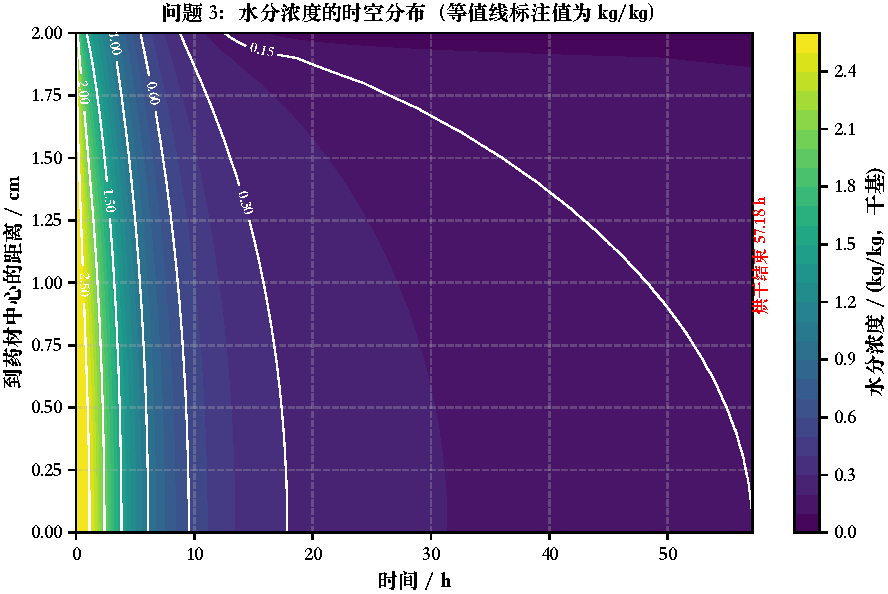
\includegraphics[width=0.49\linewidth]{figs/fig-moist-2d.pdf}%
  }{%
    \instruction{【插图缺失】未找到 \texttt{figs/fig-moist-2d.pdf}，请先运行 \texttt{make figs}。}%
  }
  \caption{问题三水分浓度的时空分布（横轴为时间、纵轴为到药材中心的距离，等值线标注值的单位为 kg/kg；红色虚线为烘干结束时刻）}
  \label{fig:q3-2d}
\end{figure}

图~\ref{fig:q3-2d} 把整个烘干过程的含水率场画在一张图上，可以清楚看到三个区域：左上方的``干燥区''（$\C<0.15$）在 $12$~h 内即从表面扩展到 $1$~cm 附近；中部的``过渡区''随着时间向内推进并逐渐变窄；右下方的``湿芯区''在 $24$~h 后才开始明显收缩，到结束时刻只剩下中心附近的窄带。整张图呈现明显的\textbf{``角点效应''}：靠近表面与长时间的组合区域含水率最低，靠近轴心与短时间的组合区域含水率最高，二者之间由一族近似平行的等值线相连。这一图形结构说明\textbf{干燥前沿是沿半径方向匀速推进的}，而不是``整体均匀失水''。

\genfig[0.60\linewidth]{figs/fig3-C-profiles.pdf}{长时间干燥下水分浓度沿半径的分布（问题三，取 $10\%$、$30\%$、$60\%$ 与 $100\%$ 干燥时长）}{fig:q3C}
\genfig[0.60\linewidth]{figs/fig3-C-history.pdf}{五个径向位置的水分浓度随时间的变化（问题三）}{fig:q3Chistory}

图~\ref{fig:q3C} 给出四个时刻的径向剖面：早期（$10\%$ 时长，约 $5.7$~h）剖面是``内部平台 $+$ 近表面陡降''；中期（$30\%$、$60\%$ 时长）剖面逐渐整体下移并趋于平直；到结束时刻剖面几乎是一条水平线（中心 $0.15$、表面 $0.0525$~kg/kg），径向差仅 $0.0975$~kg/kg。这与此前``后期由内部扩散控制''的判断一致：当内部补充速度足够慢时，断面上各点的含水率会以相同的速率缓慢下降，剖面的形状不再改变。

图~\ref{fig:q3Chistory} 从时间维度给出各位置的达标顺序：$r=2.0$~cm 的表面在 $12$~h 内就已低于 $0.15$~kg/kg，$r=1.5$~cm 在 $36$~h 附近达标，$r=1.0$~cm 在 $48$~h 后达标，而 $r=0.5$~cm 与轴心直到最后时刻才达标。因此\textbf{整个烘干时长实际上是由轴心附近最后 $0.5$~cm 的``湿芯''决定的}：从 $r=2.0$~cm 达标到轴心达标之间隔了约 $45$~h，占总时长的 $79\%$。这一观察对工艺优化有直接含义：若要缩短烘干时间，应设法提高\textbf{内部}水分的迁移能力（例如提高温度以增大扩散系数、或采用间歇式干燥让内部水分有时间重新分布），而不是单纯加大表面风速或提高表面换热强度。

\section{问题四：考虑失水收缩的烘干时长}
\label{sec:q4}

\subsection{模型的建立：移动边界与坐标系选择}
\label{sec:q4model}

问题四要求考虑药材因失水而发生的尺寸变化，经验公式改用附录 4。由附件 2，药材半径由 $2.000$~cm 收缩到末值 $1.198$~cm，即\textbf{半径减少约 $40\%$}；而附件 2 只给出半径，未给出长度与体积的变化。因此本问首先要确定``失水如何改变形状''这一题目未明确给出的几何关系。

\subsubsection{几何假设与收缩运动学}

按假设 A10，本文取\textbf{长度不变}、收缩在径向\textbf{均匀}发生：同一物质壳层按同一比例缩放，即半径为 ${\rpos}_0$ 的初始物质点在任何时刻满足

\begin{equation}
\rpos({\rpos}_0,\t)=\frac{\R(\t)}{\Rzero}\,{\rpos}_0 .
\label{eq:kinematics}
\end{equation}

``长度不变''的依据是控制方程按\textbf{单位轴向长度}写出、$\Llen$ 不进入任何一项；代价是若长度按同一比例缩短，药材体积将只剩 $21.5\%$（而非固定长度假设下的 $35.9\%$），而附件 2 的数据\textbf{无法区分这两种情形}——这是本问最大的几何不确定性。

对式\eqref{eq:kinematics} 求时间导数，得到材料点的径向速度

\begin{equation}
v(\rpos,\t)=\left.\frac{\partial \rpos}{\partial \t}\right|_{{\rpos}_0}
=\frac{\dot \R}{\Rzero}{\rpos}_0=\frac{\dot \R}{\R}\,\rpos=\xi\dot \R,
\qquad \xi:=\frac{\rpos}{\R(\t)} .
\label{eq:materialvelocity}
\end{equation}

\subsubsection{干物质守恒与干基表观密度}

单位\textbf{当前}体积内的干物质质量为 $\rho_d(\t)$。由式\eqref{eq:kinematics}，半径 $\R$ 的圆柱内干物质质量正比于 ${\R}^2$，而干物质总量守恒，故

\begin{equation}
\rho_d(\t)\R(\t)^2=\rho_d(0){\Rzero}^2
\quad\Longrightarrow\quad
\rho_d(\t)=\rho_d(0)\left(\frac{\Rzero}{\R(\t)}\right)^2 .
\label{eq:rhod}
\end{equation}
即\textbf{材料被压缩，干基表观密度随半径的平方反比增大}。该关系可用干物质连续性方程自洽检验（径向均匀收缩时 $\partial\rho_d/\partial\rpos=0$）：

\begin{equation}
\frac{\partial \rho_d}{\partial \t}+\frac{1}{\rpos}\frac{\partial(\rpos\rho_d v)}{\partial \rpos}
=-\frac{2\rho_d\dot \R}{\R}+\frac{1}{\rpos}\frac{\partial}{\partial \rpos}\left(\rho_d\frac{{\rpos}^2\dot \R}{\R}\right)
=-\frac{2\rho_d\dot \R}{\R}+\frac{2\rho_d\dot \R}{\R}=0 .
\label{eq:dmcheck}
\end{equation}

\subsubsection{固定坐标下的水分守恒方程}

以干基含水率写水分守恒：单位体积内的水质量为 $\rho_d\C$，相对材料运动的扩散通量为 $-\rho_d\Ddiff\,\partial_\rpos\C$，故

\begin{equation}
\frac{\partial(\rho_d\C)}{\partial \t}
+\frac{1}{\rpos}\frac{\partial(\rpos\rho_d\C v)}{\partial \rpos}
=\frac{1}{\rpos}\frac{\partial}{\partial \rpos}\left(\rpos\rho_d\Ddiff\frac{\partial \C}{\partial \rpos}\right).
\label{eq:fixedframe}
\end{equation}
将左端展开（注意 $\rho_d$ 与 $\rpos$ 无关）：

\begin{equation}
\rho_d\frac{\partial \C}{\partial \t}
+\C\underbrace{\left(\frac{\partial\rho_d}{\partial \t}+\frac{\rho_d}{\rpos}\frac{\partial(\rpos v)}{\partial \rpos}\right)}_{=\,0\ \text{（式}\eqref{eq:dmcheck}\text{）}}
+\rho_d v\frac{\partial \C}{\partial \rpos}
=\frac{1}{\rpos}\frac{\partial}{\partial \rpos}\left(\rpos\rho_d\Ddiff\frac{\partial \C}{\partial \rpos}\right).
\end{equation}
两端约去 $\rho_d$ 后得到\textbf{固定物理坐标下的方程}

\begin{equation}
\frac{\partial \C}{\partial \t}+v\frac{\partial \C}{\partial \rpos}
=\frac{1}{\rpos}\frac{\partial}{\partial \rpos}\left(\rpos\Ddiff\frac{\partial \C}{\partial \rpos}\right).
\label{eq:euler}
\end{equation}
注意此时\textbf{必须保留}对流项 $v\,\partial_\rpos\C$：它来自材料本身的运动，是坐标原点不动带来的表观输运。

\subsubsection{材料坐标变换与严格相消}
\label{sec:cancellation}

若直接在式\eqref{eq:euler} 上求解，就必须处理随时间移动的边界 $\R(\t)$，并解决对流项带来的 CFL 限制。本文改为引入\textbf{材料坐标} $\xi=\rpos/\R(\t)\in[0,1]$，把移动域映射到固定域。由链式法则

\begin{equation}
\left.\frac{\partial}{\partial \rpos}\right|_{\t}=\frac{1}{\R}\left.\frac{\partial}{\partial \xi}\right|_{\t},
\qquad
\left.\frac{\partial \xi}{\partial \t}\right|_{\rpos}=-\frac{\rpos\dot \R}{{\R}^2}=-\frac{\xi\dot \R}{\R},
\end{equation}

\begin{equation}
\left.\frac{\partial}{\partial \t}\right|_{\rpos}
=\left.\frac{\partial}{\partial \t}\right|_{\xi}+\left.\frac{\partial \xi}{\partial \t}\right|_{\rpos}\frac{\partial}{\partial \xi}
=\left.\frac{\partial}{\partial \t}\right|_{\xi}-\frac{\xi\dot \R}{\R}\frac{\partial}{\partial \xi}.
\label{eq:chainrule}
\end{equation}
把式\eqref{eq:chainrule} 与式\eqref{eq:materialvelocity} 代入式\eqref{eq:euler} 的左端，得到本问推导中最关键的一步：

\begin{equation}
\underbrace{\left.\frac{\partial \C}{\partial \t}\right|_{\rpos}}_{=\,{\C}_\t|_\xi-\frac{\xi\dot \R}{\R}{\C}_\xi}
+v\underbrace{\frac{\partial \C}{\partial \rpos}}_{=\,{\C}_\xi/\R}
={\C}_\t\big|_\xi-\frac{\xi\dot \R}{\R}{\C}_\xi+(\xi\dot \R)\frac{{\C}_\xi}{\R}
={\C}_\t\big|_\xi .
\label{eq:cancel}
\end{equation}

\textbf{坐标变换引入的输运项 $-\frac{\xi\dot \R}{\R}{\C}_\xi$ 与材料速度带来的对流项 $+\frac{\xi\dot \R}{\R}{\C}_\xi$ 大小相等、符号相反，恰好严格相消}。换言之，物质导数就等于固定 $\xi$ 的偏导数：

\begin{equation}
\frac{\mathrm{D}\C}{\mathrm{D}\t}
:=\left.\frac{\partial \C}{\partial \t}\right|_{\rpos}+v\frac{\partial \C}{\partial \rpos}
=\left.\frac{\partial \C}{\partial \t}\right|_{\xi}.
\end{equation}
这不是巧合：由式\eqref{eq:kinematics}，$\xi$ 被材料速度平流（$\xi_\t+v\xi_\rpos=-\frac{\xi\dot \R}{\R}+\xi\dot \R\cdot\frac1{\R}=0$），因此固定 $\xi$ 的点始终跟踪同一团材料，$\xi$ 是\textbf{材料标签}而非纯数学技巧。

右端的扩散算子作同样变换：

\begin{equation}
\frac{1}{\rpos}\frac{\partial}{\partial \rpos}\left(\rpos\Ddiff\frac{\partial \C}{\partial \rpos}\right)
=\frac{1}{{\R}^2\xi}\frac{\partial}{\partial \xi}\left(\xi\Ddiff\frac{\partial \C}{\partial \xi}\right).
\end{equation}

\subsubsection{变换后的方程组与表面条件}

综合以上结果，得到问题四在\textbf{固定计算域 $\xi\in[0,1]$} 上的控制方程组：

\begin{equation}
\boxed{\
\left.\frac{\partial \C}{\partial \t}\right|_{\xi}=\frac{1}{{\R}^2(\t)\,\xi}\frac{\partial}{\partial \xi}\left(\xi\,\Ddiff\frac{\partial \C}{\partial \xi}\right),
\qquad
\rho\cp\left.\frac{\partial \T}{\partial \t}\right|_{\xi}=\frac{1}{{\R}^2(\t)\,\xi}\frac{\partial}{\partial \xi}\left(\xi\,\kcond\frac{\partial \T}{\partial \xi}\right)
\ }
\label{eq:q4system}
\end{equation}
其中物性取附录 4（$\rho=760+90\C$、$\cp=1850+2150\wfrac$、$\kcond=0.12+0.20\wfrac$、$\Ddiff=4.2\times10^{-4}e^{-0.30/\C}e^{-3850/\T}$，$\wfrac=\C/(1+\C)$，$\T$ 用开尔文）。\textbf{与前三问相比，方程组的形式完全相同，只多出一个 $1/{\R}^2(\t)$ 的整体因子，且不含任何对流项。}物理含义是：$\xi$ 坐标下所有长度都按 $\R(\t)$ 缩放，扩散算子只被 $1/{\R}^2$ 加速；由于 $\R$ 减小，\textbf{特征扩散时间 ${\R}^2/\Ddiff$ 随之缩短}。

表面条件（$\xi=1$）由 $\partial_\rpos={\R}^{-1}\partial_\xi$ 与式\eqref{eq:robin} 给出：

\begin{equation}
\Ddiff\left.\frac{\partial \C}{\partial \xi}\right|_{\xi=1}=-\R\,\hmass\,({\C}_s-\Cinf),
\qquad
\kcond\left.\frac{\partial \T}{\partial \xi}\right|_{\xi=1}=\R\,\hconv\,(\Tinf-{\T}_s).
\label{eq:q4bc}
\end{equation}
系数中多出的 $\R$ 是把``对 $\rpos$ 的梯度''换成``对 $\xi$ 的梯度''带来的几何因子（梯度被拉长了 $1/\R$ 倍），它与方程中的 $1/{\R}^2$ 一起决定传热与失水的速率。轴心条件仍为 $\partial_\xi\T=\partial_\xi\C=0$；初值仍为式\eqref{eq:initial}（$\t=0$ 时 $\R(0)=\Rzero$，故与前三问逐字相同）。

\subsubsection{必须避免的一个错误：不得再加对流项}

式\eqref{eq:cancel} 的相消是\textbf{逐项}完成的：链式法则产生 $-\frac{\xi\dot \R}{\R}{\C}_\xi$，材料速度产生 $+\frac{\xi\dot \R}{\R}{\C}_\xi$。因此\textbf{在式\eqref{eq:q4system} 上再次添加 $\frac{\xi\dot \R}{\R}{\C}_\xi$ 这一项是重复计入}，等价于凭空引入一个不存在的相对流动，会系统性地偏移干燥速率。

只有在下列情形才需要那一项：(i) 在\textbf{固定物理坐标} $\rpos$ 上求解而边界在动（即直接用式\eqref{eq:euler}）；(ii) 假设\textbf{非均匀收缩}，此时存在径向的相对材料速度，式\eqref{eq:dmcheck} 中的相消不再成立；(iii) 用不随材料缩放的固定网格做离散。本文三种情形都不是：网格节点是材料点，故方程中不应出现对流项。判断方法是问一句``\textbf{这个模型的网格节点是材料点还是空间点}''。

\subsubsection{退化检验}

取 $\R\equiv\Rzero$（即 $\dot \R=0$），式\eqref{eq:q4system} 退化为固定域上的方程 ${\C}_\t=(\xi\Ddiff{\C}_\xi)_\xi/({\Rzero}^2\xi)$，配合 $\Ddiff{\C}_\xi|_{\xi=1}=-\Rzero\hmass({\C}_s-\Cinf)$，与前三问在缩放坐标下的形式完全一致。程序层面做了这一检验：把附件 2 的半径序列全部置为 $\Rzero$ 后，材料坐标模式与固定半径模式的右端函数\textbf{逐位相同}（差值严格为 $0$），既验证了式\eqref{eq:cancel} 的相消，也验证了实现没有多加或少加对流项。

\subsection{模型的求解}
\label{sec:q4solve}

\subsubsection{固定材料坐标网格上的离散}

由于 $\xi$ 是材料坐标（式\eqref{eq:kinematics}），在 $\xi$ 网格上离散时式\eqref{eq:q4system} 的算子结构不随时间改变，因此仍使用第~\ref{sec:mesh} 节的表面二次加密网格（式\eqref{eq:gradedmesh}）与节点中心有限体积格式，只是每个时刻都要按当时的 $\R(\t)$ 更新方程中的 $1/{\R}^2$ 因子与界面通量：

\begin{equation}
F^C_{i+1/2}=\xi_{i+1/2}\,{\Ddiff}_{i+1/2}\frac{{\C}_{i+1}-{\C}_i}{\Delta\xi_i},
\qquad
F^T_{i+1/2}=\xi_{i+1/2}\,{\kcond}_{i+1/2}\frac{{\T}_{i+1}-{\T}_i}{\Delta\xi_i},
\end{equation}
\begin{equation}
\frac{\mathrm{d}{\C}_i}{\mathrm{d}\t}=\frac{F^C_{i+1/2}-F^C_{i-1/2}}{{\R}^2V_i},
\qquad
\frac{\mathrm{d}{\T}_i}{\mathrm{d}\t}=\frac{F^T_{i+1/2}-F^T_{i-1/2}}{{\R}^2V_i\rho_i{\cp}_i},
\qquad
F^C_{\Nr-1/2}=-\R\hmass({\C}_s-\Cinf),\quad F^T_{\Nr-1/2}=-\R\hconv({\T}_s-\Tinf).
\end{equation}

时间积分沿用第~\ref{sec:time} 节的 BDF 方法，环境条件按式\eqref{eq:interp} 插值并在附件 1 的每个测量节点重启；半径 $\R(\t)$ 由附件 2 分段线性插值，且在 $\t$ 超出附件 2 的覆盖范围时直接报错而\textbf{不做外推}（本问的终点 $50.82$~h 落在数据覆盖的 $72$~h 之内，不需要外推）。此外，由于 $1/{\R}^2$ 使方程的系数随时间变化，右端函数中的 $\R$ 与 $\dot\R$ 无关（$\dot\R$ 不进入方程，见第~\ref{sec:cancellation} 节），故附件 2 的分段线性插值在节点处的导数跳变\textbf{不构成任何数值困难}——这是材料坐标建模除实现简单之外的第二个实质好处。

\subsubsection{交付映射}

导出阶段的关键是``内部解在材料坐标上、交付网格在物理坐标上''。对第 $j$ 个输出时刻，先由附件 2 得到 ${\R}_j=\R(t_j)$，把内部节点映射为物理位置 ${\rpos}_{i,j}=\xi_i{\R}_j$，再把该时刻的含水率场插值到题目要求的固定物理位置 $0,0.1,\ldots,1.9$~cm 上；落在当时药材之外的列\textbf{留空}。交付文件的末列``药材表面''取 $\xi=1$ 节点的值，它恒为有效值，与域外留空无关。以交付文件末行（$t=183000$~s，$\R=1.2000$~cm）为例：$0$~cm 与 $1.2$~cm 列的含水率为 $0.1500$ 与 $0.0525$~kg/kg，$1.3\sim1.9$~cm 共 $7$ 列留空，末列``药材表面''与 $1.2$~cm 列相同（此时两者是同一物理位置）——这一自洽性可直接用于检验交付文件的正确性。

\subsection{结果与分析}
\label{sec:q4result}

\subsubsection{烘干时长}

\begin{equation}
\boxed{\ \tend^{(\text{问题 4})}=\QFourEventS~\mathrm{s}=\QFourEventH~\mathrm{h}\ }
\end{equation}

即考虑失水收缩后，烘干时长为 \textbf{\QFourEventH~h}。事件时刻的药材半径为 $\R=\QFourEventR$~cm（由初始 $2.0000$~cm 收缩 \QFourShrinkPct\%），表面含水率为 \QFourSurfaceEnd~kg/kg，温度场仍为全场 $323.315$~K。交付文件 \texttt{result4.xlsx} 写到 \QFourLastRowS~s（即 \QFourEventH~h 之后的第一个 $60$~s 整行）。按题目表 6 格式整理的结果见表~\ref{tab:q4-moisture}。

\geninput{tab/q4_moist}{表 6 由 \texttt{make tables} 从 \texttt{results/tables/q4\\_moist.csv} 生成；末列为当时的药材表面位置。}

\subsubsection{半径收缩的结构}

\begin{figure}[!ht]
  \centering
  \IfFileExists{figs/fig-q4-shrink.pdf}{%
    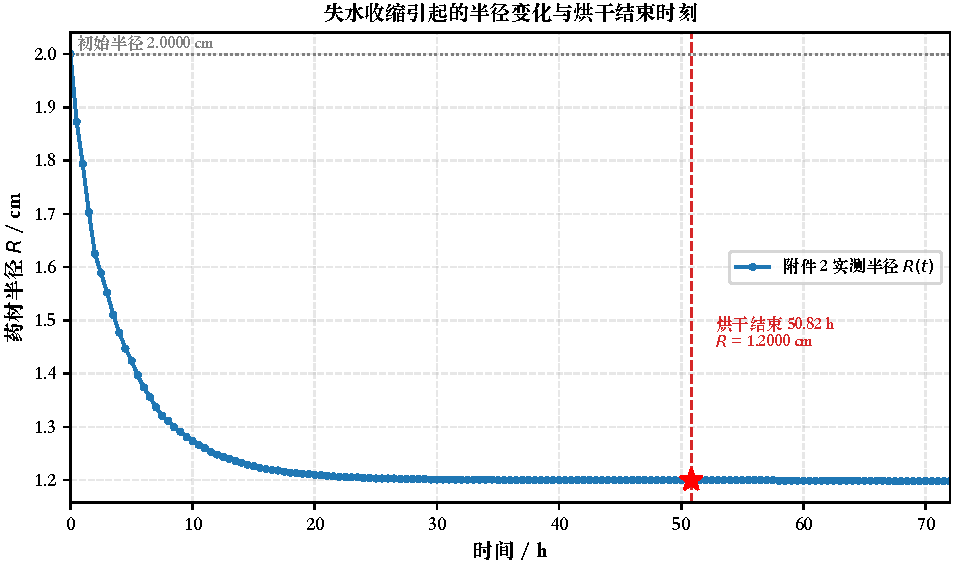
\includegraphics[width=0.45\linewidth]{figs/fig-q4-shrink.pdf}%
  }{%
    \instruction{【插图缺失】未找到 \texttt{figs/fig-q4-shrink.pdf}，请先运行 \texttt{make figs}。}%
  }
  \caption{附件 2 给出的药材半径随时间的收缩过程与烘干结束时刻（红星标出结束时刻的半径）}
  \label{fig:q4-shrink}
\end{figure}

图~\ref{fig:q4-shrink} 显示附件 2 的半径序列有三个特征。第一，\textbf{收缩主要发生在前 $3$~h}：半径由 $2.000$~cm 迅速降到约 $1.51$~cm，此后速率明显变缓；第二，$18$~h 之后半径进入近似台阶状的小幅下降，$35.0\sim57.5$~h 之间保持 $1.2000$~cm 不变；第三，\textbf{本问的烘干结束时刻 $50.82$~h 恰好落在这一平台内部}。第三点有重要的实务含义：\textbf{答案不依赖半径数据在结束时刻附近的插值细节}（该区间内 $\R$ 是常数），因此半径测量的小幅波动不会影响报出的烘干时长。同时这也说明``半径不再变化''只在小数点后两位成立：到附件 2 的末值 $1.1980$~cm 还要再降 $0.002$~cm，且发生在 $67$~h 之后。

\subsubsection{两个相反效应的分离：三个算例的对照}

由于问题三与问题四\textbf{同时}改变了物性集（附录 3 $\to$ 附录 4）与几何（固定半径 $\to$ 收缩半径），直接比较 $57.17$~h 与 $50.82$~h 无法说明收缩的作用。为此本文构造第三个算例：\textbf{同用附录 4 物性、但半径固定为 $\Rzero$}，从而把两个效应分离开。三个算例的结果如下：

\begin{table}[!ht]
  \centering
  \caption{分离参数集效应与几何效应的三个算例（B 为本文构造的对照算例，不产出交付文件）}
  \label{tab:three-cases}
  \scriptsize
  \begin{tabular}{ccccc}
    \toprule
    算例 & 物性 & 半径 & 烘干时长 / h & 用途 \\
    \midrule
    A（问题三） & 附录 3 & $\Rzero$ 固定 & $57.1694$ & 基准 \\
    B（对照算例） & 附录 4 & $\Rzero$ 固定 & \QFourFixedRadiusH & 与 A 比较即得参数集效应 \\
    C（问题四） & 附录 4 & $2.000\to\QFourEventR$~cm & \QFourEventH & 与 B 比较即得收缩效应 \\
    \bottomrule
  \end{tabular}
\end{table}

\begin{itemize}
  \item \textbf{参数集效应（A$\to$B）}：在固定几何下把物性换成附录 4 后，烘干时长由 $57.17$~h 增大到 \QFourFixedRadiusH~h，即\textbf{变慢 $2.26$ 倍}。原因是附录 4 的扩散系数前因子比附录 3 小约 $5.7$ 倍（$4.2\times10^{-4}$ 对 $2.4\times10^{-3}$），而 $\C$ 的指数由 $-0.45/\C$ 变为 $-0.30/\C$，二者共同使扩散变慢。
  \item \textbf{收缩效应（B$\to$C）}：在\textbf{同一物性集}下把半径由固定改为按附件 2 收缩，烘干时长由 \QFourFixedRadiusH~h 降到 \QFourEventH~h，即\textbf{缩短 \QFourShrinkEffectPct\%}。
  \item \textbf{净效应（A$\to$C）}：两者叠加后 $57.17$~h 变为 \QFourEventH~h，缩短 \QFourNetEffectPct\%。\textbf{这个数字是两个方向不同效应的净值，单独引用会得到误导性的结论。}
\end{itemize}

\genfig[0.70\linewidth]{figs/fig-param-comparison.pdf}{三个算例的烘干时长对照。黑色实线为问题三（附录 3、固定半径）的含水率历程，另外两条竖线分别标出对照算例（附录 4、固定半径）与问题四（附录 4、收缩半径）的终点时刻}{fig:param-comparison}

\subsubsection{为什么收缩在本模型下使干燥加快}

直觉上``半径减小 $\Rightarrow$ 水分逸出面积减小 $\Rightarrow$ 干燥变慢''，与算例 B$\to$C 的结果相反。要弄清哪一效应占优，必须把两个效应换算到同一度量上。对式\eqref{eq:q4system} 沿断面按材料测度积分（$\int_0^1(\cdot)\,\xi\,\mathrm{d}\xi$，对应离散的 $\sum_iV_i{\C}_i$），并代入表面条件式\eqref{eq:q4bc}：

\begin{equation}
\frac{\mathrm{d}}{\mathrm{d}\t}\int_0^1\C\,\xi\,\mathrm{d}\xi
=\frac{1}{{\R}^2}\left[\xi\Ddiff{\C}_\xi\right]_{\xi=0}^{\xi=1}
=\frac{\Ddiff{\C}_\xi(1)}{{\R}^2}
=-\frac{\hmass({\C}_s-\Cinf)}{\R}.
\label{eq:lossrate}
\end{equation}
即单位材料测度的失水速率为 $\hmass({\C}_s-\Cinf)/\R$。再换成单位长度药材的失水质量：由式\eqref{eq:rhod}，$\rho_d(\t){\R}^2\equiv\text{const}$，故

\begin{equation}
W=\rho_d{\R}^2\cdot2\pi\int_0^1\C\xi\,\mathrm{d}\xi
\quad\Longrightarrow\quad
\frac{\mathrm{d}W}{\mathrm{d}\t}=-2\pi\underbrace{\R}_{\text{面积因子}}\underbrace{\rho_d}_{\propto\,{\R}^{-2}}\hmass({\C}_s-\Cinf).
\label{eq:twochannels}
\end{equation}

于是两条通道各自的量纲因子为：\textbf{表面积通道}正比于 $\R$（半径减小使逸出面积变小，趋于$\cdot$变慢）；\textbf{干基密度通道}正比于 ${\R}^{-2}$（材料被压实，单位体积内的水量随半径平方反比增大，趋于变快）；两者相乘后\textbf{净表面项正比于 ${\R}^{-1}$，即趋于变快}。与此同时，\textbf{内部再分布的时间尺度正比于 ${\R}^2/\Ddiff$}，半径减小同样使它变快。

因此在本模型所采用的边界闭合下，\textbf{``面积减小''这一条并没有表现为净减速}：干基表观密度随收缩上升（式\eqref{eq:rhod}）把面积因子完全抵消并超过，两个通道都指向变快。定量地看，算例 B$\to$C 的时长比为 $50.8242/129.0926=0.394$，而 $({\R}_{\text{end}}/\Rzero)^2=(1.2000/2.0000)^2=0.360$，二者同量级；这与``内部扩散控制下时间尺度正比于 ${\R}^2/\Ddiff$''的判断一致，也说明\textbf{路径缩短占主导}。

需要明确的是，这一结论\textbf{依赖于表面传质的闭合形式}（假设 A7）。若改用``水蒸气通量正比于表面积''的另一种闭合，面积减小的效应会重新出现，结论可能改变。本文如实陈述本模型下的结论，并在第~\ref{sec:limitations} 节把它列为一项结构性限制，而不通过``在材料坐标方程里再加一个对流项''的方式人为制造``面积效应''（第~\ref{sec:cancellation} 节已论证那是重复计入）。

\genfig[0.60\linewidth]{figs/fig4-C-profiles.pdf}{含收缩时水分浓度沿材料坐标 $\xi=\rpos/\R(\t)$ 的分布（问题四）}{fig:q4C}
\genfig[0.60\linewidth]{figs/fig4-C-history.pdf}{不同径向位置的水分浓度随时间的变化（问题四，位置按固定物理距离取值）}{fig:q4Chistory}

\subsubsection{与问题三的对比}

图~\ref{fig:q4C}、图~\ref{fig:q4Chistory} 给出问题四的剖面与历程。与问题三（图~\ref{fig:q3C}、图~\ref{fig:q3Chistory}）相比有三点值得注意。

第一，\textbf{干燥曲线的形状相同、时间轴被压缩}。问题四的剖面同样经历``表层先降—前沿内推—整体趋平''三段，只是各段的时间尺度按 ${\R}^2$ 成比例缩短：问题三中表面在 $12$~h 才降到 $0.1639$~kg/kg，问题四中 $12$~h 时表面已降到 $0.1667$~kg/kg（此时半径已收缩到 $1.3740$~cm，而问题三在同一时刻的半径仍是 $2.0$~cm）；问题三中轴心在 $36$~h 为 $0.1854$~kg/kg，问题四中同一时刻为 $0.1921$~kg/kg，剖面的相对形状也与问题三基本一致。

第二，\textbf{交付表在形态上与前三问不同}。表~\ref{tab:q4-moisture} 的 $1.5$~cm 列在各时刻\textbf{均留空}：因为 $\t=6$~h 时半径已收缩到 $1.3740$~cm，固定位置 $1.5$~cm 落在药材之外。这不是数据缺失，而是``交付位置是固定物理位置、药材却在收缩''的必然结果，也是题目把末列改为``药材表面''的原因。

第三，\textbf{末期的剖面更平坦}。结束时刻问题四的中心与表面含水率分别为 $0.15$ 与 $0.0525$~kg/kg（差 $0.0975$），与问题三几乎相同；但由于此时药材只有 $1.2$~cm 半径，同样的绝对差值对应的\textbf{相对梯度更大}，这说明收缩后期内部水分向外补充的``路程''虽短，含水率的相对落差并未减小。

\section{模型检验}
\label{sec:validation}
\label{sec:evaluation}

本节按``数值可信度''与``物理结构性局限''两类分别陈述检验结果。前者回答``在给定的方程与边界下，数值解算得准不准''；后者回答``给定的方程与边界是否足以描述真实烘干过程''。两类问题不能互相替代，这一点是本节的行文原则。

\subsection{离散守恒审计}

在有限体积离散下，所有内部界面通量在总体收支中成对抵消，故含水率的总量变化必须精确等于表面传质通量的累积值。定义归一化含水率总量 $\sum_iV_i{\C}_i$ 与累积失水量，本文在每一个输出时刻检验

\begin{equation}
\sum_iV_i{\C}_i(\t)+\int_0^\t\frac{\hmass}{\R}\left[\C(\R,s)-\Cinf(s)\right]\mathrm{d}s
=\sum_iV_i{\C}_i(0),
\label{eq:massaudit}
\end{equation}
其实测相对残差为：问题一 \QOneMassError，问题二 \QTwoMassError，问题三 \QThreeMassError，问题四 \QFourMassError（网格加密各档的结果见表~\ref{tab:validation-grid}）。这些残差都在机器精度量级，说明\textbf{离散格式的质量收支是闭合的}。对问题四而言，这一检验尤其有意义：式\eqref{eq:massaudit} 是在材料测度下成立的，若式\eqref{eq:cancel} 的相消被误加或多加了对流项，或者式\eqref{eq:rhod} 的幂次写错，残差会立刻变成 $O(1)$。

能量方面的结论要谨慎一些。问题一的物性为常数，可以把 $\rho\cp$ 提出积分号，从而检验``域内显热变化 $=$ 累积对流换热''这一积分恒等式，实测相对残差为 \QOneEnergyError。问题二$\sim$四则\textbf{不能}做同样的检验：式\eqref{eq:q2system} 中的 $\rho\cp$ 随含水率变化，无法从时间导数中提出，因此$\int\rho\cp(\T-{\T}_0)\mathrm{d}V$ 并不是该方程所守恒的量。本文对这三问只检验\textbf{瞬时}收支恒等式，即每一时刻都满足

\begin{equation}
{\R}^2\sum_iV_i\,\rho_i{\cp}_i\frac{\mathrm{d}{\T}_i}{\mathrm{d}\t}=F^T_{\Nr-1/2}=\R\hconv(\Tinf-{\T}_s),
\end{equation}
并明确\textbf{不声称} $\rho\cp\T$ 的积分守恒。把问题一的积分守恒结论搬到后三问，是一个很容易犯而后果不小的错误，故在此显式区分。

\subsection{空间网格加密}
\label{sec:conv}

以 $\Nr=641,1281,2561,5121$ 四档网格求解同一问题，把结果插值到题目指定的输出网格上比较相邻两档的最大差值，结果见表~\ref{tab:validation-grid}（网格收敛与 Richardson 估计的做法见文献~\cite{roache1998}）。

\geninput{tab/validation_grid}{网格加密验证表由 \texttt{make tables} 从 \texttt{results/validation/accuracy*.json} 生成。}

由表~\ref{tab:validation-grid} 可见，相邻网格的场量差按约四倍缩小，与二阶空间离散的预期一致：问题一的最大温度差依次为 $4.82\times10^{-6}$、$1.37\times10^{-6}$、$2.89\times10^{-7}$~K（比值约 $3.5$、$4.7$），$2561$ 与 $5121$ 两档之差已小于 $3\times10^{-7}$~K 与 $2.3\times10^{-7}$~kg/kg，\textbf{远小于交付要求的四位小数分辨率}（$10^{-4}$），故正式计算取 $\Nr=2561$ 是充分的。

\textbf{其二，终点时刻对网格的依赖更弱，且收敛更快。} 问题三的终点时刻差由 $0.2137$~s 降到 $0.0534$~s 与 $0.0134$~s（相邻档比值约 $4.0$、$4.0$），问题四由 $7.0\times10^{-3}$~s 降到 $1.7\times10^{-3}$~s 与 $6.2\times10^{-4}$~s。也就是说，$\Nr$ 加倍带来的终点时刻变化在正式网格上只有 \QThreeGridEventDiff~s（问题三）与 \QFourGridEventDiff~s（问题四），\textbf{比报出的小时位数（$10^{-4}$~h $=0.36$~s）小两到三个数量级}。这从数值上支持了``烘干时长可以作为答案报出''这一主张。

\textbf{其三，终点判据本身依赖网格，但依赖很弱。} 表~\ref{tab:validation-grid} 的``终点时刻差''列同时反映了两件事：解本身的收敛，以及``全场最大值''这一泛函对网格的敏感性（网格越细，最大值越大，达标越晚）。两者在本例中都只有秒量级，故判据的网格依赖性不构成对结论的威胁。若把判据改为断面平均值，终点时刻会明显缩短，但那是另一个问题（假设 B3 已把这一选择及其代价写明）。

\subsection{时间积分精度}
\label{sec:timecheck}

为把时间误差与空间误差分离，本文做了两组检验，结果见表~\ref{tab:validation-time}。第一组在\textbf{同一空间网格}上把时间积分方法由变阶 BDF 换成五阶 Radau IIA，两者解的差异即时间方法的离散误差；第二组把相对/绝对容差各收紧十倍、最大步长减半，考察误差控制的可靠性。两种时间方法分别对应文献~\cite{ascher1998}与 SciPy 的 Radau IIA 实现~\cite{scipyradau2026}，本文使用的事件检测机制见~\cite{scipyivp2026}。

\geninput{tab/validation_time}{时间精度交叉验证表由 \texttt{make tables} 从验证报告目录 \texttt{results/validation/} 中的 JSON 文件生成。}

由表~\ref{tab:validation-time}：在 $161$ 节点网格上，两种时间方法的温度差在 $1.3\times10^{-8}\sim1.6\times10^{-8}$~K、含水率差在 $3.9\times10^{-10}\sim4.5\times10^{-10}$~kg/kg 量级，\textbf{比同一网格上的空间离散误差小两到三个数量级}，说明时间误差不是当前精度的限制因素。终点时刻的差异同样很小：问题三为 $2.06\times10^{-6}$~s、问题四为 $5.55\times10^{-4}$~s，即事件定位的可靠性远高于报出的位数要求。第二组检验（容差收紧、步长减半）给出的差异同样是场量 $10^{-6}$~K、$10^{-9}$~kg/kg、终点 $5.2\times10^{-5}$~s 量级，与第一组一致。

\begin{figure}[!ht]
  \centering
  \IfFileExists{figs/fig-validation.pdf}{%
    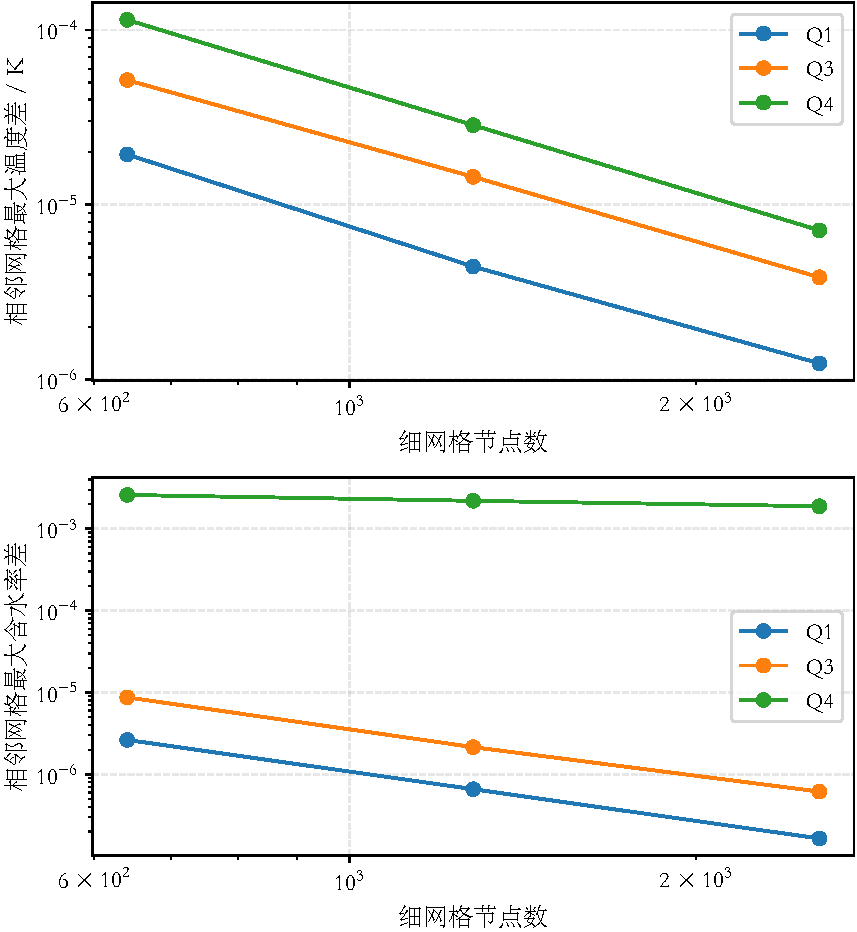
\includegraphics[width=0.68\linewidth]{figs/fig-validation.pdf}%
  }{%
    \instruction{【插图缺失】未找到 \texttt{figs/fig-validation.pdf}，请先运行 \texttt{make figs}。}%
  }
  \caption{数值验证汇总。(a) 四问的相邻网格最大温差随节点数下降，虚线为二阶参考斜率；(b) 同一网格上 BDF 与 Radau IIA 的差异；(c) 环境外推假设的灵敏度}
  \label{fig:validation}
\end{figure}

图~\ref{fig:validation}(a) 把表~\ref{tab:validation-grid} 的温度列画在双对数坐标上，四问的数据点基本平行于二阶参考线，说明\textbf{空间离散在四问中都表现出二阶收敛}；图~\ref{fig:validation}(b) 直观显示时间方法的差异比空间差异小两个数量级。

\subsection{与圆柱 Bessel 级数解析解的对照}
\label{sec:analytic}

数值解与自身的加密解比较只能说明``收敛''，不能排除``收敛到错误的方程''。为此本文为问题一的温度方程构造了独立参考解：取与环境一致的恒定环境温度与恒定的初始温度，圆柱内一维导热问题在 Robin 边界下可用 Bessel 函数级数表示

\begin{equation}
\frac{\T(\rpos,\t)-\Tinf}{{\T}_0-\Tinf}
=\sum_{n=1}^{\infty}A_n\,J_0\!\left(\mu_n\frac{\rpos}{\Rzero}\right)\exp\!\left(-\frac{\mu_n^2\alpha \t}{{\Rzero}^2}\right),
\qquad
A_n=\frac{2\,\mathrm{Bi}}{J_0(\mu_n)\left(\mu_n^2+\mathrm{Bi}^2\right)},
\label{eq:bessel}
\end{equation}
其中 $\mu_n$ 是特征方程 $\mu J_1(\mu)=\mathrm{Bi}\,J_0(\mu)$ 的正根，$\mathrm{Bi}=\hconv\Rzero/\kcond$，$\alpha=\kcond/(\rho\cp)$。由于附件 1 的环境温度是分段线性的，本文对实测驱动逐段做卷积叠加（即把分段线性驱动视为阶跃序列的叠加），从而得到一个\textbf{与数值解共享同一驱动、但计算方法完全独立}的参考解。

实测结果：模态数由 $512$ 增到 $1024$ 时参考解自身的最大变化为 \QOneBesselModes~K（即参考解已收敛到 $10^{-9}$~K 量级）；与数值解相比，最大温度误差为 \QOneBesselNTwoFiveSixOne~K（$\Nr=2561$）与 \QOneBesselNFiveOneTwoOne~K（$\Nr=5121$），$641$ 节点时为 $5.36\times10^{-6}$~K。误差随网格加密按约 $14.7$ 倍的比值下降（网格加倍约对应四倍，此处因同时收紧时间容差而更快），\textbf{这既验证了数值解正确求解了温度方程，也再次确认了空间离散的二阶性质}。这是本文最强的一项独立验证。

\subsection{物理合理性检查}

除数值精度外，本文还对解做了若干物理一致性检查，全部通过：

\begin{itemize}
  \item \textbf{含水率单调不增}：所有节点上 $\C$ 随时间是单调不增的，最大正向跳变在 $10^{-15}$ 量级（浮点舍入），未出现虚假回升；
  \item \textbf{径向单调性}：每一时刻都有 $\C$ 由轴心向表面单调递减，即干燥由表及里，与边界条件的符号方向一致；
  \item \textbf{温度不超调}：所有时刻与位置都满足 $\T\le\max_t\Tinf(\t)$，未出现高于环境温度的过冲；
  \item \textbf{环境波动引起的小幅温度回落是数据驱动而非数值不稳定}：附件 1 的实测温度序列并非单调上升（含有 $95$ 个下降步，最大单步降幅 $0.45$~K），故药材温度在 $2\sim4$~h 出现约 $10^{-3}$~K 的轻微回落；
  \item \textbf{退化检验}：问题四中把半径置为常数后，材料坐标方程与固定半径方程\textbf{逐位相同}（差值严格为 $0$），验证了式\eqref{eq:cancel} 的相消与实现的一致性；
  \item \textbf{域外留空的严格性}：问题四的交付文件中，落在当时药材之外的列必须留空、域内与表面列必须为有限值；程序对两者都做硬校验，任一条不满足即报错。
\end{itemize}

\subsection{格式与可复现性}

交付文件 \texttt{result1$\sim$4.xlsx} 的工作表名、列数、表头、时间步长与小数位数均由程序按题目模板硬校验后才写出，四个文件的实测结构为：\texttt{result1}、\texttt{result2} 各含``温度''与``水分浓度''两张工作表、$1$~s 步长；\texttt{result3}、\texttt{result4} 各含一张工作表、$60$~s 步长，\texttt{result4} 的末列是文字``药材表面''。所有数值保留四位小数。

为验证结果可复现，本文在独立目录中重新执行了完整的四问计算，并把新结果与交付文件逐单元格比较：时间列、距离列、温度场与含水率场的最大差异全部为 $0$，工作表的 XML 内容完全一致。同时，每个问题的清单文件记录了输入文件（题面、附件 1、附件 2、模板）与全部源程序的 SHA-256 摘要，以及求解所记录的运行参数，使``论文中的数字来自哪一次运行、用哪一版代码''可以追溯。

\subsection{环境外推的灵敏度分析}
\label{sec:sensitivity}

假设 B2 把 $4$~h 之后的环境条件固定为附件 1 的末值（$\Tinf=50.165~^\circ$C、$\Cinf=0.04986$~kg/kg），而这一外推覆盖了问题 2/3/4 全程约 $93\%$ 的时长。为量化其影响，本文以附件 1 末小时内 $\Tinf$、$\Cinf$ 的\textbf{实测最小值与最大值}相对末值的偏移作为扰动幅度（该偏移量本身由数据决定：附件 1 末小时内 $\Tinf$ 相对末值 $50.165~^\circ$C 的偏移为 $-0.408$~K 与 $+0.071$~K，$\Cinf$ 相对 $0.04986$~kg/kg 的偏移为 $-1.1\times10^{-4}$ 与 $+3.8\times10^{-4}$~kg/kg），重新求解并比较终点时刻。

\geninput{tab/sensitivity}{灵敏度表由 \texttt{make tables} 从 \texttt{results/validation/numerics.json} 生成。}

由表~\ref{tab:sensitivity} 可以得到三条结论。

\textbf{其一，结果对末值温度的敏感度远大于对末值含水率的敏感度。} 把末段温度整体下移 $0.408$~K 使问题三的烘干时长增加 $0.746$~h（$+1.30\%$）、问题四增加 $0.654$~h（$+1.29\%$）；而把末段含水率上下扰动 $10^{-4}$~kg/kg 量级只使终点变化 $0.002\sim0.009$~h（不足 $0.02\%$）。两者相差约两个数量级。原因是烘干时长由内部扩散控制，而扩散系数对温度是指数敏感（式\eqref{eq:app3} 的 $e^{-3850/\T}$），对边界浓度差只是线性敏感。

\textbf{其二，外推假设带来的不确定性是``小时量级''，小于模型的结构性不确定性。} 温度扰动引起的 $0.65\sim0.75$~h 是该假设下的最大偏差；而第~\ref{sec:limitations} 节列出的物理闭合问题（尤其是未计入蒸发潜热）无法用本题数据量化，且方向上是``使干燥偏快''。因此在报告结论时，应把``约 $57$~h''理解为在当前假设下的模型预测值，而不是具有小时级置信区间的实验预测。

\textbf{其三，该灵敏度分析支持``继续按末值保持外推''这一选择。} 若把末段环境温度按``最优情形''（取末小时最大值）处理，烘干时长为 $57.04$~h；按``最差情形''（取末小时最小值）为 $57.91$~h。两者与该小时的时间分辨率（题面以小时为单位报告）相比仍在同一数量级内，说明结论的定性判断（约 $2\sim2.4$ 天）不因这一外推而改变。

\subsection{模型的结构性局限}
\label{sec:limitations}

上述验证只覆盖``数值是否算准''，下列局限则属于\textbf{模型本身}，不能靠加密网格或收紧容差消除，必须如实列出：

\begin{enumerate}
  \item \textbf{表面热边界不含蒸发潜热（假设 A5）}。题目未给出水的汽化潜热与蒸发速率的关系式，本文没有凭空补一个参数，代价是表面温度可能偏高、干燥速率可能偏快。这一缺失在 $2\sim3$ 天的长时间干燥中影响明显大于 $30$~min 的预热阶段，且\textbf{其大小无法用本题数据量化}。若要评估，需要补充表面温度或蒸发速率的实测数据。
  \item \textbf{传质边界是有效闭合而非已验证的物理关系（假设 A7）}。题目给出的 $\hmass$ 与 $\Cinf$ 组合成了浓度差驱动的边界条件，但题目未说明气相水分的 kg/kg 与药材干基含水率的 kg/kg 是否同一基准（两者数值相差约 $51$ 倍）。若基准不一致，边界驱动势会整数量级地偏，烘干时长随之整体偏移。这是本文结论中不确定性最大的一环。
  \item \textbf{$4$~h 之后的环境条件是外推（假设 B2）}。该外推覆盖全程 $93\%$ 的时长，影响量级已在第~\ref{sec:sensitivity} 节量化为小时量级。
  \item \textbf{几何与收缩的简化（假设 A1、A10）}。端面效应被均摊进径向模型，无法用题目数据约束；长度不变的假设使``整块药材体积变化''这一报送口径存在两种可能（体积剩 $21.5\%$ 或 $35.9\%$），附件 2 的数据无法区分。
  \item \textbf{问题四的收缩效应结论依赖于传质闭合}。第~\ref{sec:q4result} 节得到的``收缩使干燥加快''是在``干基通量形式''的闭合下成立的；若改用按表面积的蒸气通量闭合，``面积减小''的减速效应会重新出现。本文不通过添加对流项的方式人为制造这一效应（那是重复计入，见第~\ref{sec:cancellation} 节），但也不声称该结论对闭合形式不敏感。
  \item \textbf{不引入平衡含水率（假设 A11）}。题目只给终点判据、未给吸附等温线，故本文不声称存在使干燥停滞的正平衡含水率；末期表面含水率渐近趋近但不低于 $\Cinf$，这是模型的直接后果而非物理结论。
  \item \textbf{四位小数是输出格式而非物理精度（假设 B4）}。交付文件按题目要求保留四位小数，但模型的物理预测精度受上述结构性假设限制，两者不可混淆。
\end{enumerate}

需要说明的是，第 1、2、5 条都属于\textbf{闭合关系的形式}层面：它们不改变方程的结构，也不影响数值验证的结论，但会整体平移预测值。若将来获得表面温度、气相湿度定义或吸附平衡数据，应\textbf{先修订物理闭合、再重新验证}，而不是通过加密网格来``改善''这些误差。

\section{结论}

\subsection{主要结论}

本文针对圆柱形中药材热风烘干过程，建立了圆柱坐标下一维轴对称的耦合传热--传质模型，并以统一的数值框架求解了全部四个问题。主要结论如下。

\textbf{问题一（预热平衡阶段）}：该阶段热量尚未穿透整个断面而水分变化集中在表层。经计算，$1800$~s 时药材中心与表面温度分别为 \QOneCenterT~$^\circ$C 与 \QOneSurfaceT~$^\circ$C（相差 $3.21~^\circ$C，仍低于当时环境温度 $41.51~^\circ$C），中心与表面干基含水率分别为 \QOneCenterC~kg/kg 与 \QOneSurfaceC~kg/kg（表面已失去约 $41\%$ 的初始含水率，而中心几乎未变）。温度的作用范围在 $30$~min 内已覆盖整个半径，水分的作用范围仅为表面附近约 $0.15\Rzero$（穿透深度 $0.298$~cm），因此\textbf{不能以``含水率不变''为由忽略传质，也不能对全断面施加统一的失水修正}。

\textbf{问题二（整个烘干过程）}：采用附录 3 的变物性公式后，干燥过程的时间尺度完全由传质决定：温度场在约 $4$~h 内即与环境同温（$50.165~^\circ$C）并保持均匀，而含水率要经过 $2.38$ 天才能整体达标。全过程呈现三段式规律——前 $3$~h 表层快速失水（表面降至 $1.0081$~kg/kg）、$3\sim24$~h 干燥前沿向内部推进（轴心由 $1.77$ 降到 $0.2371$~kg/kg）、$24$~h 之后全场缓慢收敛。其机制是扩散系数随含水率下降而急剧减小：由初值处的 $1.36\times10^{-8}$~m$^2$/s 降到判据值处的 $8.05\times10^{-10}$~m$^2$/s，扩散特征时间由 $8.2$~h 增大到 $138$~h。整个烘干过程历时 \textbf{\QTwoEventH~h}。

\textbf{问题三（烘干时长）}：把``药材各处含水率低于 $0.15$~kg/kg''严格解释为全场最大值判据，并把它写成只依赖时间的事件函数后，求根问题化为一次积分中的向下过零检测。求得烘干所需时间为 \textbf{\QThreeEventH~h}（\QThreeEventS~s）；交付文件写到首个严格合格的 $60$~s 采样行 \QThreeLastRowS~s（\QThreeLastRowH~h），两者相差 \QThreeGap~s，含义不同、不可混用。结果还表明\textbf{烘干时长实际上由轴心附近最后 $0.5$~cm 的湿芯决定}：表面在 $12$~h 内即已达标，而轴心到 $57.17$~h 才达标，中间相隔约 $45$~h，占总时长的 $79\%$。

\textbf{问题四（考虑失水收缩）}：由干物质守恒导出干基表观密度按 ${\R}^{-2}$ 增大，并通过材料坐标变换 $\xi=\rpos/\R(\t)$ 证明了坐标变换引入的输运项与材料速度对流项\textbf{严格相消}，从而把移动边界问题化为固定域问题且方程中不含对流项。求得烘干时长为 \textbf{\QFourEventH~h}，结束时刻的药材半径为 \QFourEventR~cm（收缩 \QFourShrinkPct\%），且该时刻落在附件 2 半径平台的内部，故答案不依赖半径数据在终点附近的插值细节。经三个算例的对照分离后：参数集由附录 3 换为附录 4 使烘干时长按 $2.26$ 倍变慢，而\textbf{收缩本身使烘干时长缩短 \QFourShrinkEffectPct\%}（$129.09$~h $\to$ $50.82$~h）；两者叠加的净效应为缩短 \QFourNetEffectPct\%。收缩使干燥加快的机制是：在内部扩散控制下（$\hmass\R/\Ddiff\approx20\sim25\gg1$），时间尺度正比于 ${\R}^2/\Ddiff$，而干基表观密度随收缩上升抵消并超过了表面积减小的影响。

四问的最终答案汇总于表~\ref{tab:answers}。

\begin{table}[!ht]
  \centering
  \caption{四个问题的最终答案汇总}
  \label{tab:answers}
  \scriptsize
  \begin{tabular}{lll}
    \toprule
    问题 & 要求 & 本文答案 \\
    \midrule
    问题 1 & $1800$~s 内温度与含水率分布 & 中心/\allowbreak 表面温度 \QOneCenterT/\QOneSurfaceT~$^\circ$C；含水率 \QOneCenterC/\QOneSurfaceC~kg/kg \\
    问题 2 & 整个烘干过程的规律 & 温度 $4$~h 内均匀化；含水率三段式下降；全程 \QTwoEventH~h \\
    问题 3 & 烘干所需时间 & \textbf{\QThreeEventH~h}（\QThreeEventS~s） \\
    问题 4 & 考虑收缩的烘干时长 & \textbf{\QFourEventH~h}（\QFourEventS~s），末半径 \QFourEventR~cm \\
    \bottomrule
  \end{tabular}
\end{table}

\subsection{结论的适用范围}

上述结论成立的前提是第~\ref{sec:assumptions} 节列出的 15 条假设，其中三条对结论的适用范围影响最大，需要在使用这些数字时一并说明：

第一，\textbf{结论适用于热风对流为主导、且干燥由内部扩散控制的工况}。本文采用纯对流的热边界（不含蒸发耗热），并对传质使用题给的浓度差闭合。若实际过程以辐射或微波加热为主，或表面蒸发由外部气流控制而非内部扩散控制，则模型结构需要更换。

第二，\textbf{烘干时长的数值带有小时量级的不确定性}。$4$~h 之后的环境条件按末值保持外推覆盖了全程 $93\%$ 的时长，按附件 1 末小时的实测波动幅度做灵敏度分析，问题三的时长在 $57.04\sim57.91$~h 之间变化（$\pm1.3\%$）；而传质基准与潜热缺失这两项结构性闭合问题的影响无法用题目数据量化，方向上会使干燥偏快。因此``约 \QThreeEventH~h''应理解为当前模型与假设下的预测值。

第三，\textbf{问题四关于收缩效应的方向性结论依赖于传质闭合形式}。本文证明在本模型采用的干基通量闭合下，收缩使干燥加快，机制与 ${\R}^2/\Ddiff$ 一致；若改用按表面积定义的蒸气通量闭合，面积减小的减速效应会重新出现。因此该结论应表述为``在本模型闭合下收缩使干燥加快''，而不宜作为一般性物理结论。

在明确以上边界后，本文的模型与结果可用于：估算给定工艺条件下的烘干时间与所需批次间隔；判断工艺瓶颈在表面换热还是内部扩散，从而指导工艺参数的调整方向（本文的分析表明瓶颈在内部扩散，故提高温度比提高风速更有效）；以及在扩展为优化问题后，用于设计升温曲线以缩短烘干时间或降低能耗。


% ---- 附录（不受 30 页限制；顺序：AI 使用说明 -> 参考文献 -> 支撑材料 -> 源程序） ----
\appendix
\section{支撑材料与复现说明}
\subsection{文件用途与运行方法}
支撑材料包为\texttt{cumcm2026A\_support.zip}。主要文件包括：\texttt{src/}下的物性、空气湿度、边界、有限体积求解及导出模块；\texttt{scripts/}下的求解、验证和图表生成入口；\texttt{tests/}下的核验程序；\texttt{results/result1.xlsx}至\texttt{result4.xlsx}、数值摘要和验证报告；\texttt{paper/}下的论文源文件、自动生成表格与矢量插图；\texttt{docs/model/}下的模型规格和文献依据。具体清单随支撑包附带，原始题目附件按目录\texttt{problem/}读取。

本次使用Python、NumPy、SciPy、pandas、openpyxl和Matplotlib完成求解与结果输出，以XeLaTeX编译中文论文。已配置环境时，在项目根目录执行：
\begin{lstlisting}[language={},numbers=none]
conda run -n 26A python scripts/run_pipeline.py
\end{lstlisting}
该入口依次生成主方案、附件拟合方案、验证报告、论文表图、源码附录、PDF与支撑包。单独计算四问可执行\texttt{python run\_all.py}；单独编译论文使用\texttt{latexmk -xelatex}，输出目录指定为\texttt{paper/build}。
所有数值先以SI单位计算，写出时再换算；论文表格从结果工作簿或同一次计算的连续终点记录读取，摘要和正文关键数字通过自动生成的宏引用。原始题目数据不修改，失败的积分和格式校验会中止计算。

\subsection{AI辅助使用说明}
本解题过程使用AI辅助核对题面与格式、检索文献、推导和审查模型、编写Python程序及组织LaTeX正文。论文中数值由本地程序实际运行得到，文献按可核验来源列示；AI生成的数值建议不直接作为结果。此次生成不包含参赛身份、学校、签名或任何提交操作。

\subsection{完整源程序}
以下源程序从项目实际文件直接载入；相同代码也以可运行的文本文件提供。论文排版中的自动换行不改变支撑包内的文件内容。
% Generated by paper/build_sources.py; source is included directly.
\subsubsection*{\texttt{run\_all.py}}
\lstinputlisting[language=Python]{../run_all.py}
\subsubsection*{\texttt{src/common/boundary.py}}
\lstinputlisting[language=Python]{../src/common/boundary.py}
\subsubsection*{\texttt{src/common/correlations.py}}
\lstinputlisting[language=Python]{../src/common/correlations.py}
\subsubsection*{\texttt{src/common/export.py}}
\lstinputlisting[language=Python]{../src/common/export.py}
\subsubsection*{\texttt{src/common/io\_excel.py}}
\lstinputlisting[language=Python]{../src/common/io_excel.py}
\subsubsection*{\texttt{src/common/numerical\_settings.py}}
\lstinputlisting[language=Python]{../src/common/numerical_settings.py}
\subsubsection*{\texttt{src/common/paths.py}}
\lstinputlisting[language=Python]{../src/common/paths.py}
\subsubsection*{\texttt{src/common/plotting.py}}
\lstinputlisting[language=Python]{../src/common/plotting.py}
\subsubsection*{\texttt{src/common/problem\_spec.py}}
\lstinputlisting[language=Python]{../src/common/problem_spec.py}
\subsubsection*{\texttt{src/common/psychrometrics.py}}
\lstinputlisting[language=Python]{../src/common/psychrometrics.py}
\subsubsection*{\texttt{src/common/radial.py}}
\lstinputlisting[language=Python]{../src/common/radial.py}
\subsubsection*{\texttt{src/common/solution.py}}
\lstinputlisting[language=Python]{../src/common/solution.py}
\subsubsection*{\texttt{src/common/units.py}}
\lstinputlisting[language=Python]{../src/common/units.py}
\subsubsection*{\texttt{src/q1/solver.py}}
\lstinputlisting[language=Python]{../src/q1/solver.py}
\subsubsection*{\texttt{src/q2/solver.py}}
\lstinputlisting[language=Python]{../src/q2/solver.py}
\subsubsection*{\texttt{src/q3/solver.py}}
\lstinputlisting[language=Python]{../src/q3/solver.py}
\subsubsection*{\texttt{src/q4/solver.py}}
\lstinputlisting[language=Python]{../src/q4/solver.py}
\subsubsection*{\texttt{scripts/\_bootstrap.py}}
\lstinputlisting[language=Python]{../scripts/_bootstrap.py}
\subsubsection*{\texttt{scripts/\_runner.py}}
\lstinputlisting[language=Python]{../scripts/_runner.py}
\subsubsection*{\texttt{scripts/audit\_q4\_boundary\_layer.py}}
\lstinputlisting[language=Python]{../scripts/audit_q4_boundary_layer.py}
\subsubsection*{\texttt{scripts/build\_paper\_assets.py}}
\lstinputlisting[language=Python]{../scripts/build_paper_assets.py}
\subsubsection*{\texttt{scripts/fit\_ambient\_temperature.py}}
\lstinputlisting[language=Python]{../scripts/fit_ambient_temperature.py}
\subsubsection*{\texttt{scripts/make\_figs.py}}
\lstinputlisting[language=Python]{../scripts/make_figs.py}
\subsubsection*{\texttt{scripts/make\_tables.py}}
\lstinputlisting[language=Python]{../scripts/make_tables.py}
\subsubsection*{\texttt{scripts/package\_delivery.py}}
\lstinputlisting[language=Python]{../scripts/package_delivery.py}
\subsubsection*{\texttt{scripts/parse\_attachments.py}}
\lstinputlisting[language=Python]{../scripts/parse_attachments.py}
\subsubsection*{\texttt{scripts/probe\_templates.py}}
\lstinputlisting[language=Python]{../scripts/probe_templates.py}
\subsubsection*{\texttt{scripts/run\_all.py}}
\lstinputlisting[language=Python]{../scripts/run_all.py}
\subsubsection*{\texttt{scripts/run\_fitted\_scenario.py}}
\lstinputlisting[language=Python]{../scripts/run_fitted_scenario.py}
\subsubsection*{\texttt{scripts/run\_pipeline.py}}
\lstinputlisting[language=Python]{../scripts/run_pipeline.py}
\subsubsection*{\texttt{scripts/run\_q1.py}}
\lstinputlisting[language=Python]{../scripts/run_q1.py}
\subsubsection*{\texttt{scripts/run\_q123\_accuracy.py}}
\lstinputlisting[language=Python]{../scripts/run_q123_accuracy.py}
\subsubsection*{\texttt{scripts/run\_q2.py}}
\lstinputlisting[language=Python]{../scripts/run_q2.py}
\subsubsection*{\texttt{scripts/run\_q3.py}}
\lstinputlisting[language=Python]{../scripts/run_q3.py}
\subsubsection*{\texttt{scripts/run\_q4.py}}
\lstinputlisting[language=Python]{../scripts/run_q4.py}
\subsubsection*{\texttt{scripts/selfcheck.py}}
\lstinputlisting[language=Python]{../scripts/selfcheck.py}
\subsubsection*{\texttt{scripts/validate\_accuracy.py}}
\lstinputlisting[language=Python]{../scripts/validate_accuracy.py}
\subsubsection*{\texttt{scripts/validate\_fitted\_scenario.py}}
\lstinputlisting[language=Python]{../scripts/validate_fitted_scenario.py}
\subsubsection*{\texttt{scripts/validate\_latent.py}}
\lstinputlisting[language=Python]{../scripts/validate_latent.py}
\subsubsection*{\texttt{scripts/verify\_accuracy\_outputs.py}}
\lstinputlisting[language=Python]{../scripts/verify_accuracy_outputs.py}
\subsubsection*{\texttt{tests/test\_accuracy.py}}
\lstinputlisting[language=Python]{../tests/test_accuracy.py}
\subsubsection*{\texttt{tests/test\_framework.py}}
\lstinputlisting[language=Python]{../tests/test_framework.py}
\subsubsection*{\texttt{tests/test\_numerics.py}}
\lstinputlisting[language=Python]{../tests/test_numerics.py}
\subsubsection*{\texttt{paper/build\_sources.py}}
\lstinputlisting[language=Python]{../paper/build_sources.py}



\end{document}
